%-----------------------------------------------
%  Engineer's Thesis
%  Warsaw University of Technology
%-----------------------------------------------

\documentclass[
    bindingoffset=5mm,
    footnoteindent=3mm,
    hyphenation=true
]{src/wut-thesis}

\graphicspath{{tex/img/}}
\addbibresource{bibliografia.bib}

%-------------------------------------------------------------
% Configuration
%-------------------------------------------------------------
\facultyeiti
\EngineerThesis
\langeng

\begin{document}

%------------------
% Title Page
%------------------
\institute{Control and Computation Engineering}
\major{Computer Science}
\specialization{Software Engineering}
\title{
    Web/desktop application (TypeScript) for visualizing and composing dependency graph between reusable software components
}
\engtitle{
    Web/desktop application (TypeScript) for visualizing and composing dependency graph between reusable software components
}
\poltitle{
    Aplikacja web/desktop (TypeScript) do wizualizacji i edycji grafu zależności pomiędzy reużywalnymi modułami oprogramowania
}
\author{Binh Vuong Le Duc}
\album{330097}
\supervisor{mgr inż. Sławomir Niespodziany}
\date{\the\year}
\maketitle

%-------------------------
% Authorship Declaration
%-------------------------
\cleardoublepage
\makeauthorship

%-------------------------
% Abstract (English)
%-------------------------
\cleardoublepage
\abstract
This thesis presents the design and implementation of a desktop application that visualizes and edits dependency graphs between reusable C++ embedded software modules. Module metadata is read from an Artifactory server or local git repositories and surfaced as a draggable catalog; the user composes the dependency graph according to project needs. The output is a topology file consumed by an existing CI/CD pipeline that builds a binary tailored to the chosen module composition. The application is implemented with Electron, React, and TypeScript, and replaces the manual JSON authoring workflow identified as future work in the framework's reference paper.

\keywords
dependency injection, visual programming, embedded systems, graph editing, Electron

%-------------------------
% Streszczenie (Polish)
%-------------------------
\cleardoublepage
\secondabstract
Niniejsza praca przedstawia projekt i implementację aplikacji desktopowej do wizualizacji i edycji grafów reprezentujących zależności pomiędzy reużywalnymi modułami oprogramowania wbudowanego napisanymi w~C++. Aplikacja odczytuje metadane modułów z~serwera Artifactory lub lokalnych repozytoriów git i prezentuje je w~formie przeciągalnego katalogu; użytkownik komponuje graf zależności zgodnie z~potrzebami projektu. Wynikiem działania są pliki topologii wykorzystywane przez istniejący potok CI/CD do zbudowania binarnej wersji aplikacji odpowiadającej wybranemu zestawowi modułów. Aplikację zaimplementowano w~technologiach Electron, React oraz TypeScript; zastępuje ona ręczne tworzenie pliku topologii w~formacie JSON, wskazane jako dalszy kierunek prac w~publikacji opisującej framework.

\secondkeywords
wstrzykiwanie zależności, programowanie wizualne, systemy wbudowane, edycja grafów, Electron

\pagestyle{plain}

%-------------------------
% Table of Contents
%-------------------------
\cleardoublepage
\tableofcontents

%-------------------------
% Chapters
%-------------------------
\cleardoublepage
\pagestyle{headings}

\clearpage
\section{Introduction}

\subsection{Motivation}
In the modern embedded systems development landscape, the cost of software exceeds the cost of designing the hardware it runs on~\cite{niespodziany2025}. As semiconductor technology advances and customer demand for broader, more sophisticated functionality grows, an embedded application is assembled by dozens of engineers across several teams, each one producing independent modules that recombine into many product variants across the device's lifetime.

The industry's response to this assembly problem is to formalize it: separate the modules from the application that consumes them, and describe their composition in a structure independent of any single module's source code. The \textit{diff} framework, presented by Niespodziany~\cite{niespodziany2025}, embodies that response for C++ embedded software through data-driven dependency injection: the application's composition is described in a JSON topology file consumed at startup.

While \textit{diff} improves reusability and flexibility, composing a product variant means editing the topology file manually. The developer must ensure its structural correctness, with limited tool support. This flow does not meet the demands of a reliable, repeatable engineering process~\cite{humble2010continuous}, and these demands grow with the size of the system.

The industry's assembly problem and the framework's own proposal~\cite{niespodziany2025} together motivate \textbf{\textit{diff-forge}}~: a visual tool that supports managing the dependency graph, and producing JSON file consumed by the existing C++ without modification. Next section sets out the specific gaps that \textit{diff-forge} aims to resolve.

\subsection{Problem Statement}
Manual maintenance of a \textit{diff} topology file imposes three major gaps along the developer's workflow. Each grows with the size of the system and the number of developers who work with the file.

\textbf{Lack of module discovery.}
Modules are distributed across Artifactory repositories, with many modules per repository and many versions per module. To compose a new system, the developer must learn which modules exist, what interfaces they expose, and what parameters they accept. This gap scales with the size of the catalog and the number of new systems assembled.

\textbf{Lack of graph readability.}
The dependency graph is encoded as text. To trace which components depend on a given module, or whether one component depends on another directly or transitively, the developer reads the JSON or runs a custom query against it. Every architectural question, from the impact of a change to the presence of a cycle, requires this reconstruction.

\textbf{Lack of real-time validation feedback.}
The JSON parser only checks syntax and is not capable of detecting lexical errors within each entry's configuration fields (such as identifiers, dependency references, parameters, \ldots), or structural errors across the JSON file (cycles, unmet dependencies, interface mismatches). These errors are caught only when the binary starts, in CI, or during code review. A broken build blocks other developers, and responsibility for fixing it often falls to someone other than the original author.

\subsection{Project Goals and Scope}
The primary goal of this project is to develop \texttt{diff-forge}, a cross-platform desktop application that enables developers to visually compose, verify, and export software topologies. The application utilizes modern web technologies including TypeScript, React~\cite{reactjs}, and Electron~\cite{electronjs}. The specific goals of the application include:
\begin{itemize}
    \item Providing an intuitive drag-and-drop interface for instantiating components from a managed catalog.
    \item Implementing a real-time validation engine to prevent structural errors before they reach the production environment.
    \item Ensuring seamless integration with existing C++ development workflows by exporting framework-compliant configuration files.
\end{itemize}

\subsection{Thesis Structure}
The following chapters comprise this thesis: Chapter~2 reviews the state of the art in dependency injection and visual programming. Chapter~3 provides an overview of the \texttt{diff} framework and its target use cases. Chapter~4 describes the architectural design of \texttt{diff-forge}, while Chapter~5 details its implementation. Lastly, Chapter~6 evaluates the tool's effectiveness, followed by concluding remarks in Chapter~7.

\clearpage
\section{Background}

This chapter establishes the technical and conceptual grounding the work rests on. Section~2.1 covers the foundations: component-based software engineering in embedded systems, the dependency injection and inversion of control patterns that the \textit{diff} framework uses to compose systems, the \textit{diff} framework itself, and the module distribution path from which it draws components. Section~2.2 reviews related work in visual composition for software systems and in cross-platform desktop application frameworks.

\subsection{Foundations}

\subsubsection{Component-Based Software Engineering in Embedded Systems}

Component-Based Software Engineering (CBSE) is the practice of building software from independent units called components, each with explicit interfaces that declare what it provides and what it requires from other components~\cite{szyperski2002}.

In an embedded system, a component is a unit like a network link driver, a timer, or a message source. Embedded products usually ship as a family of related devices that share most of their software but differ in hardware~\cite{clements2001spl}. Writing a separate codebase per device does not scale. Every shared bug fix has to be applied to every codebase, and the maintenance cost grows with the number of devices in the family. CBSE supports this setting because a component, once written, can appear in any device that needs it, and each device's software is composed from a different subset of the available components~\cite{crnkovic2002}.

CBSE on its own leaves two questions open. The first, how a component declares the other components it requires, is answered by dependency injection (\S\ref{sec:di-ioc}). The second, how the assembled system resolves those declarations into concrete instances, is answered by the \textit{diff} runtime (\S\ref{sec:diff-framework}).

\subsubsection{Dependency Injection and Inversion of Control}
\label{sec:di-ioc}

Inversion of Control (IoC) is the design principle in which a framework, rather than the component itself, decides when and how the component is instantiated and connected to its dependencies~\cite{fowler2004di}. Dependency Injection (DI) implements IoC by separating the component from the construction of its dependencies: a component declares what it requires, and an external assembler supplies it, typically through constructor parameters or setter methods.

DI changes the direction of control. Without DI, a component creates its dependencies internally:
\begin{lstlisting}[language=C++, aboveskip=10pt]
class Component {
    Database db{DatabaseFactory::create()};  // self-created
};
\end{lstlisting}

With DI, the dependencies are passed in by an external assembler:
\begin{lstlisting}[language=C++, aboveskip=10pt]
class Component {
  public:
      Component(Database& db);  // injected via constructor
  private:
      Database& db_;
};
\end{lstlisting}

The same \texttt{Component} class can take a real \texttt{Database} in production, a mock one in tests, and a different implementation when wired into a separate product variant.

\paragraph{Static vs.\ Runtime DI}
DI has two main forms, distinguished by when the wiring is resolved (Figure~\ref{fig:static-vs-runtime-di}).

\begin{figure}[ht]
    \centering
    \resizebox{\textwidth}{!}{
        \begin{tikzpicture}[
    node distance=17mm and 10mm,
    box/.style={draw, rounded corners=2pt, minimum height=10mm, text width=24mm, align=center, font=\small},
    artifact/.style={box, fill=gray!10},
    process/.style={box, fill=blue!10},
    wiring/.style={box, fill=blue!10, very thick, draw=orange!80!black},
    output/.style={box, fill=green!10},
    arr/.style={->, thick},
    arrwiring/.style={->, very thick, draw=orange!80!black},
    panel/.style={font=\small\bfseries}
]
% --- Panel A: Static DI ---
\node[panel] (titleA) {Static DI};
\node[artifact, below=4mm of titleA.south west, anchor=north west] (srcA) {Source code\\+ headers};
\node[wiring, right=of srcA] (compA) {Compiler\\(links graph)};
\node[output, right=of compA] (binA) {Wired binary};
\node[output, right=of binA] (sysA) {Live system};
\draw[arr] (srcA) -- (compA);
\draw[arr] (compA) -- (binA);
\draw[arr] (binA) -- (sysA);
\node[font=\scriptsize\itshape, color=orange!80!black, below=0.5mm of compA] {wiring resolved};

% --- Panel B: Runtime DI ---
\node[panel, below=16mm of srcA.south west, anchor=north west] (titleB) {Runtime DI};
\node[artifact, below=4mm of titleB.south west, anchor=north west] (srcB) {Source code};
\node[process, right=of srcB] (compB) {Compiler};
\node[output, right=of compB] (binB) {Generic binary};
\node[output, right=of binB] (sysB) {Live system};
\node[artifact, below=of binB] (jsonB) {JSON\\description};
\draw[arr] (srcB) -- (compB);
\draw[arr] (compB) -- (binB);
\draw[arrwiring] (binB) -- node[above, font=\scriptsize\itshape, color=orange!80!black]{loader} (sysB);
\draw[arrwiring] (jsonB) -- node[midway, sloped, above, font=\scriptsize\itshape, color=orange!80!black]{wiring resolved} (sysB);
\end{tikzpicture}

    }
    \caption{Static DI vs.\ runtime DI.}
    \label{fig:static-vs-runtime-di}
\end{figure}

\textbf{Static DI} resolves wiring at compile time: a header or template specialisation names the concrete type for each interface, the compiler links the graph, and the resulting binary has no wiring step at startup. The compiler rejects unfilled dependencies, so the system is verifiable. The binary contains exactly one topology, so every variant requires a rebuild.

\textbf{Runtime DI} resolves wiring at process startup from a data description (XML, JSON, YAML). The same binary takes different descriptions and produces different systems, so one build serves multiple variants. The compiler no longer checks the wiring, so a malformed description fails only when the runtime loader executes it.

\paragraph{DI in C++14}
relies on template metaprogramming and static initialisation. C++ has no reflection-based DI container like Java or C\#, so frameworks build their own using the Curiously Recurring Template Pattern~\cite{coplien1995}. C++14~\cite{cpp14standard} adds variadic templates and stronger \texttt{constexpr} support that simplify this construction. Niespodziany~\cite{niespodziany2025} details how the \textit{diff} framework (\S\ref{sec:diff-framework}) applies these techniques.

\FloatBarrier

\subsubsection{The \textit{diff} Framework}
\label{sec:diff-framework}

The \textit{diff} framework~\cite{niespodziany2025} is a runtime DI implementation for C++14 embedded software. Figure~\ref{fig:diff-workflow} sketches its end-to-end workflow: component classes are compiled into the binary and register themselves before \texttt{main()} runs, then a JSON topology file drives the construction of a live system. The examples below come from \textit{diff\_broker}, the reference application that ships with the framework.

\begin{figure}[ht]
    \centering
    \resizebox{\textwidth}{!}{
        \begin{tikzpicture}[
    node distance=6mm and 8mm,
    box/.style={draw, rounded corners=2pt, minimum height=9mm, text width=34mm, align=center, font=\small, inner sep=2pt},
    source/.style={box, fill=gray!10, text width=24mm},
    registry/.style={box, fill=orange!20, draw=orange!80!black, thick},
    process/.style={box, fill=blue!10},
    output/.style={box, fill=green!10, text width=28mm},
    arr/.style={->, thick},
    dasharr/.style={->, thick, dashed, draw=orange!80!black},
    phase/.style={font=\small\bfseries\itshape, anchor=west},
    every node/.append style={execute at begin node={\hyphenpenalty=10000\exhyphenpenalty=10000}}
]
% --- Phase 1: static-init (before main) ---
\node[phase] (phaseA) at (0,0) {Compile + static-init};

\node[source, below=2mm of phaseA.south west, anchor=north west] (cls) {Component\\classes};
\node[registry, right=22mm of cls] (factreg) {FactoryRegistry};
\draw[arr] (cls) -- node[above, font=\scriptsize\itshape]{registered} (factreg);

% --- Phase 2: runtime (in main) ---
\node[phase, below=16mm of phaseA.south west, anchor=north west] (phaseB) {Runtime};

\node[source, below=2mm of phaseB.south west, anchor=north west] (topo) {topology.json};
\node[process, right=of topo] (loader) {TopologyLoader};
\node[process, right=of loader] (build) {\texttt{diff::Build}};
\node[registry, right=of build] (depreg) {DependencyRegistry};
\node[output, below=8mm of depreg] (app) {Application\\\texttt{\scriptsize build.get<I>()}};

\draw[arr] (topo) -- (loader);
\draw[arr] (loader) -- (build);
\draw[arr] (build) -- (depreg);
\draw[arr] (depreg) -- (app);

% --- Cross-phase: FactoryRegistry feeds Build ---
\draw[dasharr] (factreg.south) -- ++(0,-8mm) -| (build.north) node[pos=0.25, above, font=\scriptsize\itshape, color=orange!80!black] {lookup by type};
\end{tikzpicture}

    }
    \caption{The \textit{diff} workflow. Component classes register their factories at static-initialisation time. At runtime, the framework reads the topology JSON, looks up the factories by type name, and instantiates the components into a live application accessible by interface.}
    \label{fig:diff-workflow}
\end{figure}

\paragraph{Components and interface components}
Niespodziany~\cite{niespodziany2025} distinguishes two kinds of components. A regular \textit{component} implements algorithms and data structures. An \textit{interface component} is header-only: a pure-virtual C++ class that declares an interface and lives in its own translation unit so no implementation can leak detail across the contract. A component class inherits from \texttt{diff::Component<T, ...>}, where \texttt{T} is the class itself and the remaining template parameters declare which interfaces the component provides. Listing~\ref{lst:diff-component} shows \texttt{LinkGsm}: it implements \texttt{ILink} and exposes itself under that interface, so any later component that needs an \texttt{ILink} can be wired to it.

\begin{addmargin}[0mm]{0mm}
\begin{lstlisting}[language=C++, caption={A \textit{diff} component that implements the \texttt{ILink} interface.}, label=lst:diff-component, aboveskip=10pt]
// ILink.h -- interface component (header-only)
class ILink {
public:
    virtual ~ILink() = default;
    virtual bool send(const std::string& message) = 0;
};

// LinkGsm.h
class LinkGsm : public diff::Component<LinkGsm, diff::as<ILink>> {
public:
    LinkGsm();
    bool send(const std::string& message) override;
};
\end{lstlisting}
\end{addmargin}

\paragraph{The topology file}
The system's wiring is described by a JSON \textit{topology} file. Each entry carries the component's type name, a unique instance id, the ordered ids of the dependencies that should be injected into the constructor, and a typed configuration map (Listing~\ref{lst:topology-entry}). The framework instantiates the entries in order, so the topology must be in dependency order: every component appears after all the components it depends on.

\begin{addmargin}[0mm]{0mm}
\begin{lstlisting}[caption={Topology entry consumed by the \textit{diff} loader at startup.}, label=lst:topology-entry, aboveskip=10pt]
{
  "type": "MessageSource",
  "id": "msgSrc0",
  "version": "1.0.0",
  "source": "https://artifactory.example.com/artifactory/diff",
  "dependencies": ["linkEth0", "linkGsm0"],
  "config": {
    "count": 3,
    "content": "Diff says hello."
  }
}
\end{lstlisting}
\end{addmargin}

\paragraph{Topology as a data product}
The same compiled binary, given two different topology files, produces two different running systems with different components and different wiring. This is what Niespodziany~\cite{niespodziany2025} calls \textit{data-driven} composition. A new variant is a JSON edit, not a code change. The trade-off is that the JSON file becomes the primary artifact of the system, and any error in it shows up only when the loader runs. That trade-off is what motivates the visual editor presented in this thesis.

\subsubsection{Module Distribution: Conan and Artifactory}

C++ has no standard package manager, so teams pick one of several third-party tools to manage binary dependencies. \textbf{Conan}~\cite{conan} is the one used by the \textit{diff} ecosystem: a package manager that builds and consumes C++ libraries through \textit{recipes}, build scripts that describe how to compile, package, and install a library. A Conan package is identified by \texttt{name/version@user/channel} and may carry pre-built binaries for multiple compilers, architectures, and build types.

\textbf{Artifactory}~\cite{artifactory} is a binary repository manager from JFrog that, among other formats, supports the Conan protocol. Teams publish their internal C++ libraries as Conan packages to an Artifactory repository, and consumer projects fetch them through standard Conan tooling. In a \textit{diff}-based environment, each component is a Conan package, and each package carries a catalog entry that describes the component to potential consumers: the interfaces it implements, the dependencies it requires, and the configuration parameters it accepts. Listing~\ref{lst:catalog-entry} shows the catalog entry for a \texttt{MessageSource} component.

\begin{addmargin}[0mm]{0mm}
\begin{lstlisting}[caption={Catalog entry for the \texttt{MessageSource} component, published alongside its Conan package.}, label=lst:catalog-entry, aboveskip=10pt]
{
  "type": "MessageSource",
  "version": "1.0.0",
  "implements": ["IProcessable"],
  "requires": [
    { "slot": "link",    "type": "ILink" },
    { "slot": "backup",  "type": "ILink", "isArray": true }
  ],
  "config": {
    "count":   { "type": "uint32", "min": 1, "max": 1000 },
    "content": { "type": "string", "default": "msg" }
  }
}
\end{lstlisting}
\end{addmargin}

The catalog entry is a \textit{schema} rather than an instance: \texttt{implements} lists the interfaces the component provides, \texttt{requires} describes the slots that must be filled by other components (each with a name, an interface type, and an \texttt{isArray} flag for multi-binding slots), and \texttt{config} declares each parameter's type, allowed range, and default value. A topology entry (\S\ref{sec:diff-framework}) is a concrete \textit{instance} of a catalog entry: it picks an \texttt{id}, fills each \texttt{requires} slot with the \texttt{id} of another instance, and assigns concrete values inside \texttt{config}.

For \textit{diff-forge}, the catalog of available modules is the set of catalog entries hosted on Artifactory. At startup, the tool queries the repository's Conan API, downloads each component's catalog entry, and presents the entries in the side panel. The ingestion pipeline is described in \S4.3.

\subsection{Related Work}

\subsubsection{Visual Composition for Software Systems}

Visual composition tools let developers build software by arranging and connecting nodes on a canvas, replacing or supplementing textual code. The approach has a long history in domain-specific environments. LabVIEW~\cite{labview} uses a dataflow paradigm for instrumentation and measurement software. Simulink~\cite{simulink} applies it to control-system modelling. Node-RED~\cite{nodered} offers a flow-based editor for IoT devices and web services. Unreal Engine's Blueprint system~\cite{blueprint} exposes game-engine APIs as a visual scripting language.

In all of these tools, the canvas is a directed graph. Nodes represent units of computation or component instances. Edges represent dataflow or dependency. The two graph-theory concepts relevant to \textit{diff-forge} are the directed acyclic graph and the algorithm for ordering its nodes.

\paragraph{Directed Acyclic Graph (DAG)}
is a finite directed graph that contains no directed cycles~\cite{cormen2009}. Each edge has a direction, and no sequence of edges returns to its starting node. DAGs are the natural model for dependency relationships in software. Each component depends on zero or more others, and a cycle would mean a component transitively depends on itself. A topology with a cycle cannot be instantiated, because no component in the cycle has all of its dependencies available.

The \textit{diff} framework requires the topology to be a DAG. The loader refuses to instantiate a topology that contains a cycle. \textit{diff-forge} enforces the DAG property at export time. When the user attempts to export a topology that contains a cycle, the validation engine rejects it and points at the cycle's edges.

\paragraph{Topological Sorting}
produces a linear ordering of a DAG's nodes such that for every directed edge $(u, v)$, $u$ comes before $v$~\cite{cormen2009}. For a dependency graph, a topological order is a valid construction sequence. Every component's dependencies appear before the component itself.

Kahn's algorithm~\cite{kahn1962} computes a topological order in linear time (Figure~\ref{fig:kahn-algorithm}). It begins with the set of nodes that have no incoming edges. At each step, it removes one such node from the set, appends it to the output, and reduces the in-degree of each neighbour. Any neighbour that drops to zero in-degree joins the set. The algorithm terminates when the set is empty. If all nodes have been emitted, the output is a valid topological order. If some nodes remain unemitted, the graph contains a cycle.

\begin{figure}[ht]
    \centering
    \resizebox{\textwidth}{!}{
        \begin{tikzpicture}[
    node/.style={circle, draw, thick, minimum size=0.8cm, fill=white},
    arrow/.style={->, thick},
    stepbox/.style={rectangle, draw, dashed, inner sep=0.3cm, fill=gray!5}
]

% Step 1
\begin{scope}[local bounding box=s1]
    \node[node, fill=green!10] (1a) {1};
    \node[node, fill=green!10, right=1cm of 1a] (2a) {2};
    \node[node, below=0.8cm of 1a] (3a) {3};
    \node[node, right=1cm of 3a] (4a) {4};
    \draw[arrow] (1a) -- (3a);
    \draw[arrow] (2a) -- (3a);
    \draw[arrow] (3a) -- (4a);
    \node[below=0.1cm of 3a, xshift=0.5cm] {\small \textbf{Step 1:} Find nodes with in-degree 0 (1, 2)};
\end{scope}

% Step 2
\begin{scope}[shift={(6,0)}, local bounding box=s2]
    \node[node, opacity=0.3] (1b) {1};
    \node[node, opacity=0.3, right=1cm of 1b] (2b) {2};
    \node[node, fill=green!10, below=0.8cm of 1b] (3b) {3};
    \node[node, right=1cm of 3b] (4b) {4};
    \draw[arrow, opacity=0.3] (1b) -- (3b);
    \draw[arrow, opacity=0.3] (2b) -- (3b);
    \draw[arrow] (3b) -- (4b);
    \node[below=0.1cm of 3b, xshift=0.5cm] {\small \textbf{Step 2:} Remove 1, 2. Node 3 in-degree $\to$ 0};
\end{scope}

% Step 3
\begin{scope}[shift={(12,0)}, local bounding box=s3]
    \node[node, opacity=0.3] (1c) {1};
    \node[node, opacity=0.3, right=1cm of 1c] (2c) {2};
    \node[node, opacity=0.3, below=0.8cm of 1c] (3c) {3};
    \node[node, fill=green!10, right=1cm of 3c] (4c) {4};
    \draw[arrow, opacity=0.3] (1c) -- (3c);
    \draw[arrow, opacity=0.3] (2c) -- (3c);
    \draw[arrow, opacity=0.3] (3c) -- (4c);
    \node[below=0.1cm of 3c, xshift=0.5cm] {\small \textbf{Step 3:} Remove 3. Node 4 in-degree $\to$ 0};
\end{scope}

% Final Result
\node[below=1.5cm of s2, align=center, fill=yellow!10, draw, thick] {
    \textbf{Final Topological Order:}\\
    $[1, 2, 3, 4]$
};

\end{tikzpicture}

    }
    \caption{Step-by-step topological sorting using Kahn's algorithm.}
    \label{fig:kahn-algorithm}
\end{figure}

\textit{diff-forge} uses Kahn's algorithm during export. The topology JSON file requires entries to appear in load-compatible order (leaves before roots). Kahn's algorithm produces this order from the canvas graph (\S4.5).

\subsubsection{Cross-Platform Desktop Application Frameworks}

A cross-platform desktop application framework lets a single codebase target Windows, macOS, and Linux without per-platform rewrites. The candidates differ along three dimensions. The first is the rendering technology, either a web stack or native widgets. The second is the language used for application logic. The third is the deployment profile, such as binary size and memory footprint. Table~\ref{tab:cross-platform} summarises the most active frameworks at the time of writing.

\begin{table}[ht]
\centering
\caption{Cross-platform desktop application frameworks compared. Figures are typical for a minimal application bundled for production distribution.}
\label{tab:cross-platform}
\footnotesize
\begin{tabular}{lllll}
\toprule
\textbf{Framework} & \textbf{Renderer} & \textbf{App Language} & \textbf{Binary Size} & \textbf{Memory Footprint} \\
\midrule
Electron       & Chromium + Node.js & TypeScript / JavaScript & 100--200 MB & 200--500 MB \\
Tauri          & Native WebView     & Rust + TypeScript       & 10--30 MB   & 50--150 MB  \\
Qt (Widgets)   & Native widgets     & C++                     & 40--100 MB  & 50--200 MB  \\
.NET MAUI      & Native + WebView   & C\# / XAML              & 50--100 MB  & 100--300 MB \\
Flutter Desktop & Skia              & Dart                    & 30--60 MB   & 80--200 MB  \\
\bottomrule
\end{tabular}
\end{table}

\textbf{Electron}~\cite{electronjs} bundles a Chromium browser and a Node.js runtime. The application UI is written as a standard web page, and the Node.js backend provides access to OS-level APIs. The two-process architecture (main process plus renderer process) and the IPC layer between them are described in \S5.2. The trade-off is binary size and memory footprint, both larger than native alternatives.

\textbf{Tauri}~\cite{tauri} uses the OS-provided WebView (WebKit on macOS, WebView2 on Windows, WebKitGTK on Linux) for the UI and Rust for the backend. This achieves an order-of-magnitude reduction in binary size and memory at the cost of a less uniform rendering surface across platforms.

\textbf{Qt}~\cite{qt} is the long-standing C++ framework for native desktop applications. The Widgets module produces compact, native-looking applications. The QML/Quick module offers a declarative UI with hardware acceleration. The trade-off is that the application logic is written in C++, which limits the available ecosystem of UI libraries compared to the web stack.

\textbf{.NET MAUI}~\cite{maui} is Microsoft's cross-platform framework. It combines native widgets and embedded WebViews under a C\#/XAML programming model. Its primary target is mobile (Android and iOS) with desktop support as a secondary use case.

\textbf{Flutter Desktop}~\cite{flutter} uses Google's Skia renderer to draw all UI elements directly. The result is a consistent look across platforms at the cost of not matching native conventions. Its primary language is Dart.

For \textit{diff-forge}, Electron with React and TypeScript was selected (\S4.1). Familiarity with the web stack and the maturity of the React Flow canvas library~\cite{react_flow} outweighed the binary-size cost.

\input{tex/3-framework}
\clearpage
\section{Architecture and Design}

This chapter turns the architecture drivers from \S\ref{sec:arch-drivers} into a concrete design. \S\ref{sec:tech-selection} justifies the technology stack the rest of the design assumes. \S\ref{sec:hex-arch} determines the hexagonal layering of the codebase and the dependency rule that protects it. \S\ref{sec:catalog-ingestion} to \S\ref{sec:validation-engine} take the four largest design problems the drivers raise (catalog ingestion, canvas interaction, topology I/O, structural validation) and describe how each is solved at the design level.

\subsection{Technology Selection}
\label{sec:tech-selection}

The technology stack is fixed by three drivers from \S\ref{sec:arch-drivers}: AD-2, AD-1, and the canvas requirement of FR-2.x with NFR-1.2. The candidate frameworks were compared in \S\ref{sec:cross-platform-frameworks}. Table~\ref{tab:tech-selection} records the choice made at each layer and the driver each choice answers.

\begin{table}[ht]
\centering
\caption{Technology choices for \textit{diff-forge} and the architecture drivers they answer.}
\label{tab:tech-selection}
\footnotesize
\begin{tabular}{lll}
\toprule
\textbf{Layer} & \textbf{Choice} & \textbf{Primary driver} \\
\midrule
Application shell        & Electron 42              & AD-2 \\
Main-process runtime     & Node.js 22 LTS           & AD-2 \\
Renderer language        & TypeScript 5.8 (strict)  & AD-1 \\
UI framework             & React 19                 & AD-2 \\
Canvas library           & React Flow 12            & FR-2.x, NFR-1.2 \\
State management         & Zustand 5                & AD-1 \\
Component primitives     & Material UI 7            & NFR-3.x \\
Schema validation        & Zod 3                    & AD-1, AD-5 \\
Build tooling            & Vite 6 + pnpm 10         & NFR-4.3 \\
Test stack               & Vitest, Playwright       & NFR-4.3 \\
\bottomrule
\end{tabular}
\end{table}

\paragraph{Electron and TypeScript.}
The application is built on Electron with TypeScript. The first reason is practical as the author is already familiar with TypeScript and web application developement. TypeScript brings two things the tool leans on. The UI ecosystem is mature with broad library support, above all React Flow (\S\ref{sec:canvas-model}) and Zod.

The analysis in \S\ref{sec:cross-platform-frameworks} also shows that Electron is a suitable framework for cross-platform applications with a browser renderer, which can be leveraged during development. Electron's larger binary and heavier runtime are the trade-off, but the tool still meet the targets in \S\ref{sec:nfrs} as a single developer workstation tool.

\paragraph{React Flow for the canvas.}
The canvas is built on React Flow~\cite{react_flow}. In the early stage of the project, a custom canvas was written from scratch that drew the nodes, edges, and port connections. It proved inefficient on two counts. It took a large amount of time to build, and its performance did not meet NFR-1.2 as the graph grew. React Flow already gives a tuned node-and-edge user interface and the extension points the design needs: custom node and edge types and a callback that checks a connection as it is drawn (\S\ref{sec:canvas-model}), so the tool adopted it instead.

\paragraph{Zustand for state.}
The renderer keeps its state in Zustand stores~\cite{zustand}. AD-1 needs state we can test without rendering React, and a Zustand store is a plain object whose actions are ordinary functions, so a test calls them and checks the result directly. It is a small, modern library that keeps the state layer easy to read and to maintain, which is what a tool this size needs.

\paragraph{Zod for runtime schema.}
Both the catalog (from Artifactory) and the topology files (from disk) are loaded into the tool as untyped JSON. Zod gives a unified schema to check them before the core logic uses them. This includes the runtime check and the TypeScript type (\texttt{z.infer<typeof schema>}), so the parsed data cannot drift from the type the code expects. \S\ref{sec:catalog-impl} and \S\ref{sec:topology-impl} apply the same schema on read and on write.

\paragraph{Linting and the CI/CD pipeline.}
As required by NFR-4.3, ESLint carries the lint rules, including a rule that keeps renderer-only modules out of the main process, and Prettier formats the code and orders the imports by layer. The checks run at two points: a pre-commit hook is the fast local guard, and the continuous-integration pipeline runs the same checks on a clean machine and is the authoritative one. \S\ref{sec:project-structure} details the concrete configuration.

\subsection{Hexagonal Architecture}
\label{sec:hex-arch}
AD-1 requires core logic and side-effectful code to live in separate layers, with the core testable on its own. The codebase meets this with a hexagonal (ports-and-adapters) architecture~\cite{cockburn2005hexagonal}. Six layers surround the core (Figure~\ref{fig:layers}), and the dependency rule runs one way, from the outside in.

\begin{figure}[H]
    \centering
    \resizebox{0.92\textwidth}{!}{
        \begin{tikzpicture}[
    font=\small,
    box/.style={draw, rounded corners=2pt, align=center, text width=32mm, minimum height=15mm, fill=white},
    edge/.style={-{Stealth}, thick},
    lbl/.style={font=\scriptsize, fill=white, inner sep=1.5pt}
]
\node[box] (view) {\textbf{View}\\[2pt]\scriptsize canvas, catalog panel, topbar, welcome};
\node[box, below=9mm of view]     (state)     {\textbf{State +}\\\textbf{orchestration}\\[2pt]\scriptsize stores, cross-store commands};
\node[box, below=9mm of state]    (adapters)  {\textbf{Adapters}\\[2pt]\scriptsize Artifactory, cache, workspace, \\ topology, IPC client};
\node[box, below=9mm of adapters] (contracts) {\textbf{Contracts}\\[2pt]\scriptsize catalog source, cache, host API};

\draw[edge] (view)     -- node[lbl]{imports}    (state);
\draw[edge] (state)    -- node[lbl]{imports}    (adapters);
\draw[edge] (adapters) -- node[lbl]{implements} (contracts);

\node[box, text width=26mm,
      fit={($(view.north)+(-58mm,0)$) ($(contracts.south)+(-32mm,0)$)}] (core)
      {\textbf{Core}\\[2pt]\scriptsize catalog, graph,\\ topology, workspace};

\draw[edge] (view.west)      -- node[lbl]{imports} (core.east |- view.west);
\draw[edge] (state.west)     -- node[lbl]{imports} (core.east |- state.west);
\draw[edge] (adapters.west)  -- node[lbl]{imports} (core.east |- adapters.west);
\draw[edge] (contracts.west) -- node[lbl]{imports} (core.east |- contracts.west);

\node[box, right=30mm of adapters] (main) {\textbf{Main process}\\[2pt]\scriptsize OS bridge: window, typed bridge, main-side adapters};
\draw[edge] (adapters.east) -- node[lbl, above]{inter-process call} (main.west);
\end{tikzpicture}

    }
    \caption[The hexagonal layering of \textit{diff-forge}.]{The hexagonal layering of \textit{diff-forge}.}
    \label{fig:layers}
\end{figure}

\paragraph{Layer responsibilities.}
\begin{itemize}
    \item \textbf{Core.} Catalog merging, graph operations, topology serialisation, validation rules, and the workspace validity decision. No framework imports and no side effects, so every rule here is exercised by a unit test.
    \item \textbf{Contracts.} The interfaces an adapter must satisfy: a catalog source, a catalog cache, and the host API the renderer calls. A contract names a shape, not an implementation.
    \item \textbf{Adapters.} The concrete implementations of the contracts: the Artifactory-backed catalog source, the on-disk cache, the workspace and topology I/O, and the renderer-side client that forwards each call to the main process.
    \item \textbf{State and orchestration.} The in-memory stores for the graph state, the catalog status, the current workspace, the transient UI, and the notification queue, plus a thin command layer that composes several stores for a single user action.
    \item \textbf{View.} The React components, grouped into the major surfaces: canvas, catalog panel, topbar, welcome screen, and layout shell.
    \item \textbf{Main process.} The operating-system side: window lifecycle, the typed bridge, and the main-side adapters the renderer cannot hold directly.
\end{itemize}

\paragraph{}
Every arrow in Figure~\ref{fig:layers} points inward, toward the core. Each layer imports only the layers beneath it, and the core imports nothing from the project but the schema library. This direction is, for the most part, a convention the codebase follows. An ESLint \texttt{no-restricted-imports} rule~\cite{eslint} also guards the process boundary, keeping the renderer-only modules out of the main process, so the two processes do not couple by accident.

\paragraph{}
The renderer and the main process are different operating-system processes. The boundary between them is the host-API contract: the renderer holds a client adapter that forwards each call across it, a thin preload bridge exposes that call, and the main process answers it with the real adapter on its side.

\paragraph{}
The core logic is further divided into four bounded contexts (Figure~\ref{fig:bounded-contexts}). The \textit{catalog} context owns the published component metadata and the search and filter operations over it. The \textit{graph} context owns the in-memory representation of the canvas state. The \textit{topology} context owns the JSON wire format and the bidirectional translation between graph and topology. The \textit{workspace} context owns the launch directory, its validation, and the rule for what counts as a usable workspace. Cross-context references are few and explicit.

\begin{figure}[H]
    \centering
    \resizebox{0.85\textwidth}{!}{
        \begin{tikzpicture}[
  font=\small,
  ctx/.style={draw, rounded corners=3pt, align=center, text width=27mm, minimum height=18mm, fill=white},
  dep/.style={-{Stealth}, thin},
  dlbl/.style={font=\scriptsize, fill=white, inner sep=1.5pt}
]
\node[ctx] (catalog) {\textbf{Catalog}\\[2pt]\scriptsize component metadata, merge, search, filter};
\node[ctx, right=26mm of catalog] (graph)    {\textbf{Graph}\\[2pt]\scriptsize nodes, edges, config, operations, validation};
\node[ctx, right=26mm of graph]   (topology) {\textbf{Topology}\\[2pt]\scriptsize JSON wire format, graph and topology translation};
\node[ctx, below=14mm of graph]   (workspace){\textbf{Workspace}\\[2pt]\scriptsize launch directory, validity decision};

\draw[dep] (graph.west)    -- node[dlbl, above]{slots from}   (catalog.east);
\draw[dep] (topology.west) -- node[dlbl, above]{nodes, edges} (graph.east);

\node[font=\itshape, above=5mm of graph] {Core};
\end{tikzpicture}

    }
    \caption[Bounded contexts inside the core.]{Bounded contexts inside the core. The graph context is the only one with state-shape responsibility (nodes, edges, configuration values). The other three are core transformations over their respective types.}
    \label{fig:bounded-contexts}
\end{figure}

\FloatBarrier

\subsection{Catalog Ingestion Pipeline}
\label{sec:catalog-ingestion}
AD-4 demands that authoring continue when the catalog server is unreachable. The pipeline therefore treats the network and the on-disk cache as two sources for the same data and returns the latest available. Figure~\ref{fig:catalog-pipeline} traces the path across four domains. The editor requests the catalog, the main process fans the request out to every configured repository in parallel, and each repository falls back to its own cache slice on failure; the surviving slices then merge into one catalog, and the renderer learns which slices are fresh and which are stale.

\begin{figure}[H]
    \centering
    \resizebox{0.95\textwidth}{!}{
        \begin{tikzpicture}[
    font=\small,
    box/.style={draw, rounded corners=2pt, minimum height=8mm, text width=30mm, align=center},
    fe/.style={box, fill=blue!10},
    be/.style={box, fill=orange!12},
    ext/.style={box, fill=violet!12},
    env/.style={box, fill=gray!12, text width=38mm},
    cache/.style={box, fill=yellow!18},
    dec/.style={diamond, draw, aspect=2.2, inner sep=1pt, fill=orange!12, font=\scriptsize, align=center},
    arr/.style={-{Stealth}, thick},
    ret/.style={-{Stealth}, thick, dashed}
]
\newcommand{\sw}[1]{\tikz[baseline=-0.5ex]\node[draw, minimum width=3.5mm, minimum height=2.5mm, inner sep=0pt, fill=#1]{};}

\node[env] (envv) {\texttt{ARTIFACTORY\_REPOS}\\\texttt{ARTIFACTORY\_TOKEN}};
\node[be, below=12mm of envv] (handler) {Catalog request handler};
\node[be, below=6mm of handler] (source)  {Catalog source:\\fan-out per repository};
\node[dec, below=8mm of source] (dec) {fresh\\fetch ok?};
\node[be,    below=16mm of dec, xshift=-26mm] (ok)       {use fresh data,\\write cache};
\node[cache, below=16mm of dec, xshift=26mm]  (fallback) {read cache slice\\(mark stale)};
\node[be, below=38mm of dec] (merge)   {merge slices};
\node[be, below=6mm of merge] (outcome) {outcome};
\node[ext, right=16mm of source] (rest) {Artifactory, Conan v2 REST:\\search, revisions,\\export tarball, metadata};
\node[cache, right=16mm of fallback] (store) {per-component\\on-disk cache};
\node[fe, left=20mm of handler] (boot)  {Editor boot / Refresh};
\node[fe, left=20mm of outcome] (panel) {Catalog panel\\(ready, or stale / error notice)};

\draw[arr] (boot) -- (handler);
\draw[arr] (envv) -- (handler);
\draw[arr] (handler) -- (source);
\draw[arr] (source) -- node[above, font=\scriptsize]{fetch} (rest);
\draw[arr] (source) -- (dec);
\draw[arr] (dec) -- node[near start, left, font=\scriptsize]{yes} (ok);
\draw[arr] (dec) -- node[near start, right, font=\scriptsize]{no} (fallback);
\draw[arr] (fallback) -- (store);
\draw[arr] (ok)       |- (merge);
\draw[arr] (fallback) |- (merge);
\draw[arr] (merge) -- (outcome);
\draw[ret] (outcome) -- node[above, font=\scriptsize]{IPC return} (panel);

\node[draw, rounded corners=2pt, anchor=north west, font=\scriptsize, align=left, inner sep=2mm]
  at ($(panel.south west)+(0,-8mm)$) {
  \sw{blue!10}\,frontend (renderer) \quad \sw{orange!12}\,backend (main process) \quad \sw{violet!12}\,external API \\[2pt]
  \sw{gray!12}\,system env \quad \sw{yellow!18}\,on-disk cache
  };
\end{tikzpicture}

    }
    \caption[Catalog ingestion across four domains.]{Catalog ingestion across four domains. Fetch and fall-back are decided per repository, so one repository's outage does not block the rest; the merge runs over the in-memory results, and only a fresh fetch updates the cache.}
    \label{fig:catalog-pipeline}
\end{figure}

\paragraph{}
The configured repository URLs and an access token are read once from the environment (\texttt{ARTIFACTORY\_REPOS} and \texttt{ARTIFACTORY\_TOKEN}). Each URL is queried in parallel and its published metadata validated against the catalog schema (the concrete fetch is in \S\ref{sec:catalog-impl}). A repository that returns a network or parse error does not abort the load; the pipeline reads that repository's slice from the cache and marks it \textit{stale}. A repository that fetches cleanly is \textit{ok}, and one with neither a fresh fetch nor a cache hit is \textit{failed}.

\paragraph{}
A fresh fetch is always attempted first; on success the pipeline rewrites that repository's cache slice one component at a time. The merge runs over the in-memory results rather than the on-disk cache, so the editor renders before any disk write happens and a failed cache write cannot corrupt the catalog the user sees in this session. Per-repository results reduce to one of four outcomes that the renderer pattern-matches. Table~\ref{tab:catalog-outcomes} lists the scenario that produces each outcome and how the editor responds.

\begin{table}[H]
\centering
\caption[Catalog-load outcomes and the editor's response.]{Catalog-load outcomes: the scenario that produces each and how the editor responds.}
\label{tab:catalog-outcomes}
\footnotesize
\begin{tabular}{l p{5.4cm} p{4.6cm}}
\toprule
\textbf{Outcome} & \textbf{When it occurs} & \textbf{Editor response} \\
\midrule
Ready        & Every repository fetched fresh.                                          & Catalog opens; no warning. \\
Partial      & At least one slice is usable (fresh or stale) and at least one failed.    & Catalog opens; the topbar warns and names the failed repositories. \\
Error        & No repository produced data, by fresh fetch or by cache.                  & Welcome screen with a retry. \\
Unconfigured & No repository URLs were set in the environment.                          & Welcome screen explains how to set them. \\
\bottomrule
\end{tabular}
\end{table}

\FloatBarrier

\subsection{Canvas Interaction Model}
\label{sec:canvas-model}

The canvas is where the integrator does the authoring work. Four interactions matter: dropping a catalog entry to create a node, drawing an edge between two ports, editing a node's configuration in place, and selecting and deleting parts of the graph. Each follows the same shape (Figure~\ref{fig:canvas-interaction}). The split keeps the canvas thin and moves every rule into a core function tested without a browser.

\begin{figure}[H]
    \centering
    \resizebox{0.78\textwidth}{!}{
        \begin{tikzpicture}[
    node distance=7mm and 16mm,
    box/.style={draw, rounded corners=2pt, minimum height=10mm, text width=36mm, align=center, font=\small, fill=white},
    dec/.style={diamond, draw, aspect=2, inner sep=1pt, fill=white, font=\scriptsize, align=center},
    arr/.style={-{Stealth}, thick},
    ret/.style={-{Stealth}, thick, dashed},
    note/.style={font=\scriptsize\itshape, align=center}
]
\node[box] (event) {Canvas event\\\scriptsize drop $\cdot$ connect $\cdot$ edit $\cdot$ delete};
\node[box, below=of event] (handler) {Interaction handler};
\node[dec, below=8mm of handler] (dec) {valid?};
\node[box, below=10mm of dec] (commit) {State commit\\\scriptsize (apply mutation, mark dirty)};
\node[box, below=of commit] (render) {Re-render canvas};
\node[box, right=22mm of dec] (reject) {Rejected,\\no change};

\draw[arr] (event) -- (handler);
\draw[arr] (handler) -- node[right, font=\scriptsize]{candidate change} (dec);
\draw[arr] (dec) -- node[left, font=\scriptsize]{yes} (commit);
\draw[arr] (dec) -- node[above, font=\scriptsize]{no} (reject);
\draw[arr] (commit) -- (render);
\draw[ret] (render.east) -| ($(reject.east)+(8mm,0)$) |- (event.east);

\node[note, left=14mm of dec, text width=30mm] {Core logic decision: \\ ports that edge can connect to are highlighted and the rest are dimmed, before release};
\end{tikzpicture}

    }
    \caption[The shared canvas-interaction shape.]{The shared canvas-interaction shape. A UI event becomes a candidate change; the core decision accepts it (commit and re-render) or rejects it (no change).}
    \label{fig:canvas-interaction}
\end{figure}

\paragraph{Drop to create.}
Dragging a catalog tile onto the canvas creates a node. The drop is accepted only when it carries a diff-component payload, which keeps stray text or file drags from creating nodes, and the payload is re-validated against the catalog schema before anything is built. The new node takes a unique instance identifier (the type name plus the next free index), input and output ports built from the component's required and provided interfaces, and its declared default configuration.

\paragraph{Connect to wire.}
An edge runs from a provider port to a consumer port. The validity rule is a single core decision: the two slots must exist, point the right way (out to in), agree on interface type, hold at most one incoming edge on a non-array consumer slot, and not form a self-loop.

\paragraph{Edit in place.}
A node renders compact or expanded, and the expanded body holds its configuration fields. Expansion is a presentation concern held outside the graph, so a collapsed and an expanded node export the same JSON. A configuration edit is constrained at the input as the integrator types (\S\ref{sec:validation-engine}), without blocking the keystroke.

\paragraph{Pan, zoom, select, delete.}
Panning, zooming, and single or marquee selection are the canvas's direct-manipulation defaults. Keyboard shortcuts cover delete, select-all, and a momentary pan toggle. Deleting a node cascades to the edges that referenced it; the cascade is a core rule, covered by unit tests rather than left to the event handler.

\FloatBarrier

\subsection{Topology Export and Import}
\label{sec:topology-io}
AD-5 makes one round trip a hard constraint. A file exported by \textit{diff-forge} must load in the existing \textit{diff} loader unchanged, and a file re-opened by \textit{diff-forge} must rebuild the same graph that wrote it, apart from node positions, which the file does not carry. Export and import therefore round-trip the topology semantics over one wire format: the component set, the dependency wiring, and the configuration.

\textit{diff-forge} writes the topology format from \S\ref{sec:diff-framework}, with one addition for multi-binding: an array slot emits a nested array of identifiers in its dependency field, a non-array slot a single one. Entries stay in dependency order, every component after the ones it depends on.

\pagebreak

\begin{figure}[H]
    \centering
    \begin{subfigure}[t]{0.48\textwidth}
        \centering
        \resizebox{\textwidth}{!}{\begin{tikzpicture}[
    node distance=6mm and 12mm,
    box/.style={draw, rounded corners=2pt, minimum height=8mm, text width=34mm, align=center, font=\small},
    renderer/.style={box, fill=blue!10},
    pure/.style={box, fill=green!12},
    validator/.style={box, fill=red!10},
    main/.style={box, fill=orange!15},
    decision/.style={diamond, draw, aspect=2.4, inner sep=1pt, fill=white, font=\scriptsize, align=center},
    arr/.style={-{Stealth}, thick}
]
\node[renderer] (trigger) {Export};
\node[validator, below=9mm of trigger] (valid) {structural validation};
\node[decision, below=7mm of valid] (ok) {graph\\valid?};
\node[pure, below=9mm of ok] (ser) {serialise in dependency\\order (Kahn)};
\node[main, below=6mm of ser] (save) {write file (main process)};
\node[renderer, below=6mm of save] (confirm) {confirm (notification)};

\node[validator, right=14mm of ok] (flag) {flag offending nodes,\\no file written};

\draw[arr] (trigger) -- (valid);
\draw[arr] (valid) -- (ok);
\draw[arr] (ok) -- node[font=\scriptsize, right]{yes} (ser);
\draw[arr] (ok) -- node[font=\scriptsize, above]{no} (flag);
\draw[arr] (ser) -- (save);
\draw[arr] (save) -- (confirm);
\end{tikzpicture}
}
        \caption{Export.}
        \label{fig:export-pipeline}
    \end{subfigure}
    \hfill
    \begin{subfigure}[t]{0.48\textwidth}
        \centering
        \resizebox{\textwidth}{!}{\begin{tikzpicture}[
    node distance=6mm and 12mm,
    box/.style={draw, rounded corners=2pt, minimum height=8mm, text width=34mm, align=center, font=\small},
    renderer/.style={box, fill=blue!10},
    pure/.style={box, fill=green!12},
    validator/.style={box, fill=red!10},
    main/.style={box, fill=orange!15},
    decision/.style={diamond, draw, aspect=2.4, inner sep=1pt, fill=white, font=\scriptsize, align=center},
    arr/.style={-{Stealth}, thick}
]
\node[renderer] (trigger) {Import};
\node[main, below=8mm of trigger] (read) {read project file};
\node[decision, below=7mm of read] (exists) {file\\present?};
\node[pure, below=9mm of exists] (parse) {parse + shape-check};
\node[decision, below=7mm of parse] (valid) {valid?};
\node[pure, below=9mm of valid] (recon) {reconstruct graph\\(slots, config, layout)};
\node[renderer, below=6mm of recon] (render) {render on canvas};

\node[renderer, right=14mm of exists] (fresh) {fresh-workspace\\notice};
\node[validator, right=14mm of valid] (err) {error, names the path};

\draw[arr] (trigger) -- (read);
\draw[arr] (read) -- (exists);
\draw[arr] (exists) -- node[font=\scriptsize, right]{yes} (parse);
\draw[arr] (exists) -- node[font=\scriptsize, above]{no} (fresh);
\draw[arr] (parse) -- (valid);
\draw[arr] (valid) -- node[font=\scriptsize, right]{yes} (recon);
\draw[arr] (valid) -- node[font=\scriptsize, above]{no} (err);
\draw[arr] (recon) -- (render);
\end{tikzpicture}
}
        \caption{Import.}
        \label{fig:import-pipeline}
    \end{subfigure}
    \caption[Topology export and import pipelines.]{Topology I/O pipelines. (a) Export pipeline with structural-validation. (b) Import pipeline with topology parsing logic.}
    \label{fig:topology-io-pipelines}
\end{figure}

\paragraph{Export.}
The export pipeline (Figure~\ref{fig:export-pipeline}) starts when the integrator requests a save. The structural validator (\S\ref{sec:validation-engine}) runs first and refuses the export on any failure, with the offending nodes flagged and no file written. On a valid graph, a core function serialises the entries in dependency order (Kahn's algorithm, \S2.2.1) and the main process writes the file, after which a notification names the file.

\paragraph{Import.}
The import pipeline (Figure~\ref{fig:import-pipeline}) is triggered at project startup or when user switching to new valid workspace. The editor reads the project file by the exporter's naming convention. A valid file is reconstructed entry by entry: each becomes a node with its type looked up in the catalog, its slots regenerated, its configuration copied, and the node placed by topological depth so the graph reads left to right. Edges follow from the dependency lists, and the reconstructed graph renders on the canvas.

A topology may contain a component type no longer in the catalog, because the publisher retired the module or the file belongs to another project. Reconstruction keeps such a node, marks it unknown, and draws it in a distinct frame with a warning rather than refusing the whole file.

\FloatBarrier

\pagebreak

\subsection{Validation}
\label{sec:validation-engine}
AD-3 splits validation into two phases that run on different triggers.

\paragraph{Per-field validation, on canvas change.}
Each component's configuration schema declares, for every parameter, a type, an optional range, and a default. The editor turns that declaration into a typed input control, so the value is constrained as the integrator types it (a number field carries the parameter's range, a text field its maximum length) without blocking the keystroke.

\paragraph{Structural validation, at export.}
The structural check runs once, when the integrator asks to save, and treats the graph as a whole. It either passes or refuses the export with a list of offenders. Three failure classes are recognised:

\begin{itemize}
    \item \textbf{Cycle.} A dependency chain returns to its start, so no dependency order exists. The nodes in the cycle are named.
    \item \textbf{Unfilled required slot.} A required single-binding slot has no incoming edge. The node and the slot are named.
    \item \textbf{Type-mismatched edge.} A provider's interface does not match the slot it feeds. The canvas blocks this at connection time, so the export check is defence in depth.
\end{itemize}

A duplicate instance identifier is not a structural class; it is prevented at edit time, since new nodes are auto-numbered and a rename that would collide is rejected.

\begin{figure}[H]
    \centering
    \resizebox{0.9\textwidth}{!}{
        \begin{tikzpicture}[
    font=\small,
    state/.style={draw, rounded corners=3pt, minimum height=9mm, text width=30mm, align=center, fill=white},
    dec/.style={diamond, draw, aspect=2.2, inner sep=1pt, align=center, font=\scriptsize, fill=white},
    arr/.style={-{Stealth}, thick},
    ret/.style={-{Stealth}, thick, dashed},
    lbl/.style={font=\scriptsize, fill=white, inner sep=1pt},
    trig/.style={font=\scriptsize\itshape}
]
\node[state] (edit) {Editing on canvas};

% Per-field branch (left): runs on every config edit, non-blocking
\node[dec, below left=16mm and 20mm of edit] (pf) {value\\in range?};
\node[state, below=14mm of pf] (flagged) {Field flagged\\(red input)};

% Structural branch (right): runs at export, blocking
\node[dec, below right=16mm and 20mm of edit] (st) {graph\\valid?};
\node[state, below=14mm of st] (written) {File written,\\graph clean};
\node[state, below=12mm of written] (blocked) {Export blocked,\\nodes flagged};

% Triggers
\draw[arr] (edit) -- node[trig, above left]{config edit} (pf);
\draw[arr] (edit) -- node[trig, above right]{export request} (st);

% Per-field outcomes (forward)
\draw[arr] (pf) -- node[lbl, left]{no} (flagged);

% Structural outcomes (forward)
\draw[arr] (st) -- node[lbl, left]{yes} (written);
\draw[arr] (written) -- node[lbl, left]{no} (blocked);

% Returns to edit, routed orthogonally around the outside.
% Left side: two return lanes at increasing distance from the centre.
\draw[ret] (pf.west) -| node[lbl, below, pos=0.2]{yes} ($(flagged.west)+(-12mm,26mm)$) |- (edit.west);
\draw[ret] (flagged.west) -| node[lbl, below, pos=0.2]{valid edit} ($(flagged.west)+(-20mm,0)$) |- ($(edit.west)+(0,3mm)$);

% Right side: two return lanes at increasing distance from the centre.
\draw[ret] (written.east) -| node[lbl, below, pos=0.2]{reopen} ($(blocked.east)+(10mm,26mm)$) |- (edit.east);
\draw[ret] (blocked.east) -| node[lbl, below, pos=0.2]{fix and retry} ($(blocked.east)+(20mm,0)$) |- ($(edit.east)+(0,3mm)$);

\node[trig, below=4mm of blocked, text width=40mm, align=center]
    {cycle, unfilled required slot, or type-mismatched edge};
\end{tikzpicture}

    }
    \caption[The two-trigger validation state machine.]{The two-trigger validation state machine.}
    \label{fig:validation-outcome}
\end{figure}

\FloatBarrier


\clearpage
\section{Implementation}

This chapter walks through the implementation that gives the design its shape. \S5.1 covers the project structure and the tooling that holds it together. \S5.2 to \S5.7 step through the implementations of the six design problems from Chapter~4 in the same order: the IPC contract, catalog ingestion, graph state management, canvas rendering, topology I/O, and the validation engine. \S5.8 covers the workspace lifecycle, the user-interface shell that ties everything together, and the keyboard bindings.

\subsection{Project Structure and Tooling}
\label{sec:project-structure}

The source tree lays one folder per layer from \S\ref{sec:hex-arch}. Listing~\ref{lst:src-tree} shows the top of the tree at the time of writing.

\begin{addmargin}[0mm]{0mm}
\begin{lstlisting}[caption={Top-level layout of \texttt{diff-forge/src/}.}, label=lst:src-tree, aboveskip=10pt]
src/
  core/                  pure TypeScript logic
  contracts/             contract interfaces
  adapters/              contract implementations
  state/                 Zustand stores + cross-store commands
  components/            React tree
    canvas/              nodes, edges, hooks, the React Flow shell
    catalog/             left-side catalog panel
    topbar/              workspace chip, save, help, hotkey reference
    welcome/             initial-launch screen + workspace picker
    layout/              MainLayout, InitialLayout, NotificationHost
  electron/              main process + preload (the IPC bridge)
  styles/, assets/       MUI theme and static assets
  testing/               in-memory test doubles and fixtures
  App.tsx                renderer root (boot effects, layout choice)
  main.tsx               React entry point
\end{lstlisting}
\end{addmargin}

\paragraph{}
Each layer has a TypeScript path alias (\texttt{@core}, \texttt{@adapters}, \texttt{@state}, and so on) declared once and shared by the bundler and the test runner. The ESLint \texttt{no-restricted-imports} rule is keyed on those aliases to guard the process boundary (\S\ref{sec:hex-arch}). A pre-commit hook (husky) runs the linter, the formatter, and the unit suite over the staged change before a commit is allowed.

\paragraph{}
Additionally, the codebase is driven by a small set of \texttt{pnpm} scripts covering the development loop, the production build, and the common CI tasks (type-check, lint, test). Table~\ref{tab:pnpm-scripts} lists the most-used ones.

\begin{table}[ht]
\centering
\caption[Most-used \texttt{pnpm} scripts.]{Most-used \texttt{pnpm} scripts.}
\label{tab:pnpm-scripts}
\footnotesize
\begin{tabular}{ll}
\toprule
\textbf{Script} & \textbf{Effect} \\
\midrule
\texttt{pnpm dev}        & Vite + Electron with hot reload (\texttt{VITE\_DEV\_SERVER\_URL} set) \\
\texttt{pnpm build}      & \texttt{tsc} type-check then \texttt{vite build} for renderer and main \\
\texttt{pnpm test}       & Vitest, unit + component tests (no Electron, no real network) \\
\texttt{pnpm test:e2e}   & Playwright drives the packaged Electron app end-to-end \\
\texttt{pnpm typecheck}  & \texttt{tsc --noEmit}, fast feedback in CI \\
\texttt{pnpm lint}       & ESLint over \texttt{src/}, including the layer-boundary rules \\
\texttt{pnpm dist}       & \texttt{electron-builder} packages the Linux \texttt{.deb} artifact \\
\bottomrule
\end{tabular}
\end{table}

\subsection{Inter-Process Communication Contract}
\label{sec:ipc-contract}

The renderer and the main process run as separate OS processes. They cannot share a TypeScript runtime, so the only thing they can both see is a wire contract. That contract is a single TypeScript type, \texttt{HostApi}, declared once in \texttt{src/contracts/IpcContract.ts} and exported to both sides.

\paragraph{The contract type.}
\texttt{HostApi} is a nested namespace per concern. Listing~\ref{lst:hostapi} shows the current shape: four namespaces (\texttt{workspace}, \texttt{dialog}, \texttt{topology}, \texttt{catalog}) and six methods. Each method returns a promise of a typed outcome.

\begin{addmargin}[0mm]{0mm}
\begin{lstlisting}[language=, caption={The IPC contract type.}, label=lst:hostapi, aboveskip=10pt]
type HostApi = {
  workspace: {
    status:     () => Promise<WorkspaceStatus>
    openAtPath: (
      payload: { path: string }
    ) => Promise<OpenWorkspaceOutcome>
  }
  dialog: {
    openWorkspace: () => Promise<OpenWorkspaceOutcome>
  }
  topology: {
    export: (
      payload: { topology: string }
    ) => Promise<TopologyExportOutcome>
    load:   () => Promise<TopologyLoadOutcome>
  }
  catalog: {
    load: () => Promise<CatalogLoadOutcome>
  }
}
\end{lstlisting}
\end{addmargin}

\paragraph{The renderer side.}
A lightweight preload script wraps each \texttt{HostApi} method in an \texttt{ipcRenderer.invoke} call and exposes the collection as \texttt{window.electronAPI} via the \texttt{contextBridge}. Renderer adapters then wrap \texttt{electronAPI} and implement the contract interfaces detailed in \S\ref{sec:hex-arch}, ensuring that UI components and application state never interact directly with IPC channel names.

\paragraph{The main side.}
\texttt{electron/main.ts} is the only file that registers IPC handlers. On \texttt{app.ready} it constructs the production adapters once and registers one handler per channel (Listing~\ref{lst:mainipc}). Constructing the adapters once keeps the catalog and the workspace as long-lived singletons.

\begin{addmargin}[0mm]{0mm}
\begin{lstlisting}[language=, caption={Workspace IPC registration. Adapters are constructed once and each handler is a pass-through.}, label=lst:mainipc, aboveskip=10pt]
app.on('ready', () => {
  const workspaceStore = createFsWorkspaceStore(
    { getMainWindow: () => mainWindow }
  )

  ipcMain.handle(
    'workspace:status',     
    () => workspaceStore.getStatus()
  )
  ipcMain.handle(
    'topology:export',      
    (_, p) => workspaceStore.saveTopology(p.topology)
  )

  createWindow()
})
\end{lstlisting}
\end{addmargin}

\paragraph{A call across the boundary.}
Figure~\ref{fig:export-sequence} follows one contract call from the renderer to the main process. The renderer hands a single typed value, the serialised topology, to the preload bridge, which forwards it across to the handler that does the work.
\begin{figure}[H]
    \centering
    \resizebox{\textwidth}{!}{
        \begin{tikzpicture}[
    font=\scriptsize,
    head/.style={draw, rounded corners=2pt, fill=white, text width=26mm, minimum height=11mm, align=center, anchor=north},
    life/.style={dashed, gray},
    call/.style={-{Stealth}, thick},
    msg/.style={font=\scriptsize, align=center, fill=white, inner sep=1pt},
    side/.style={font=\scriptsize\itshape, align=center}
]
% Lifeline heads share one top edge (anchor=north at y=0) so messages stay horizontal.
\def\sp{34mm}
\node[head] (b) at (0*\sp, 0) {\texttt{exportTopology}\\\scriptsize renderer command};
\node[head] (c) at (1*\sp, 0) {\texttt{electronAPI}\\\scriptsize preload bridge};
\node[head] (d) at (2*\sp, 0) {\texttt{ipcMain}\\handler};
\node[head] (e) at (3*\sp, 0) {\texttt{FsWorkspaceStore}\\\scriptsize main-side adapter};

\def\botY{-50mm}
\foreach \n in {b,c,d,e}{
    \draw[life] (\n.south) -- (\n.south |- 0,\botY);
}

% Process boundary: one dashed vertical rule between preload (c) and main (d).
\coordinate (pb) at ($(c)!0.5!(d)$);
\draw[dashed, thick] (pb |- 0,4mm) -- (pb |- 0,\botY);
\node[side, fill=white, inner sep=2pt] at (pb |- 0,7mm) {process boundary};

\def\rA{-20mm}\def\rB{-31mm}\def\rC{-42mm}%

% the one typed contract call
\draw[call] (b.center |- 0,\rA) -- node[msg, above]{\texttt{topology.export(\{topology\})}} (c.center |- 0,\rA);
% crosses the boundary
\draw[call] (c.center |- 0,\rB) -- node[msg, above]{\texttt{invoke('topology:export')}} (d.center |- 0,\rB);
% only the main side touches the disk
\draw[call] (d.center |- 0,\rC) -- node[msg, above]{\texttt{saveTopology}} (e.center |- 0,\rC);
\node[side, anchor=north east] at ($(e.center |- 0,\rC)+(0,-2mm)$) {writes the file\\(only the main side\\reaches the disk)};
\end{tikzpicture}

    }
    \caption[An export request crossing the process boundary.]{An export request crossing the process boundary.}
    \label{fig:export-sequence}
\end{figure}

\paragraph{Security boundary.}
The browser window is created with \texttt{nodeIntegration: false} and \texttt{contextIsolation: true}~\cite{electronjs}. Renderer code cannot reach Node APIs directly, the isolation NFR-6.1 requires, and the only way into the main process is one of the six methods registered above. Adding a new capability is a two-file change: add the method to \texttt{HostApi} (and its outcome type), then register the corresponding handler in \texttt{main.ts}. The renderer adapter is typed against \texttt{HostApi}, so a call that drifts from the contract fails to compile. The preload bridge and the main-side registration use string-keyed channels, caught by the end-to-end tests rather than the compiler.

\FloatBarrier

\subsection{Catalog Ingestion}
\label{sec:catalog-impl}

The design in \S\ref{sec:catalog-ingestion} fans out a parallel fetch over the configured Artifactory URLs, falls back to a per-component on-disk cache when a repository fails, and returns one of four outcomes (\textit{ready}, \textit{partial}, \textit{error}, \textit{unconfigured}). Figure~\ref{fig:catalog-classes} shows the types involved and the pure functions that connect them: the Conan-side fragment becomes a validated \texttt{CatalogComponent}, a drop turns that component into a \texttt{GraphNode}, and the component's declared requirements become the node's ports.

\begin{figure}[H]
    \centering
    \resizebox{0.96\textwidth}{!}{
        \begin{tikzpicture}[
    font=\scriptsize,
    class/.style={draw, rectangle split, rectangle split parts=2, fill=green!8, text width=34mm, align=left},
    wire/.style={draw, rectangle split, rectangle split parts=2, fill=violet!8, text width=32mm, align=left},
    gnode/.style={draw, rectangle split, rectangle split parts=2, fill=blue!8, text width=32mm, align=left},
    dep/.style={-{Stealth}, dashed, thick},
    comp/.style={{Diamond[open]}-{Stealth}, thick},
    lbl/.style={font=\scriptsize\itshape, align=center}
]
\node[wire] (frag) {\textbf{ComponentFragment}
    \nodepart{two} type, version\\ implements[], requires[]\\ config \quad \textit{(Conan)}};
\node[class, right=30mm of frag] (comp) {\textbf{CatalogComponent}
    \nodepart{two} type, version, source\\ implements: string[]\\ requires: \{slot, type, isArray\}\\ config: field map};
\node[gnode, right=30mm of comp] (gn) {\textbf{GraphNode}
    \nodepart{two} id, instanceId\\ position, configData\\ slots: Slot[]};
\node[class, below=14mm of comp] (slot) {\textbf{Slot}
    \nodepart{two} name, type\\ direction: in $|$ out\\ isArray};

\draw[dep] (frag) -- node[lbl, above]{fragmentTo-\\Component} (comp);
\draw[dep] (comp) -- node[lbl, above]{createNode-\\FromCatalog} (gn);
\draw[dep] (comp) -- node[lbl, right]{buildSlots} (slot);
\draw[comp] (gn.south) |- (slot.east);

\end{tikzpicture}

    }
    \caption[Catalog types and the functions that connect them.]{Catalog types and the pure functions that connect them, from the Conan-side fragment to a node on the canvas.}
    \label{fig:catalog-classes}
\end{figure}

\paragraph{}
\texttt{CatalogSchema.ts} declares the catalog entry as a Zod schema, and the TypeScript type comes from the same declaration with \texttt{z.infer} (Listing~\ref{lst:catalog-schema}). Every parse of an external JSON, from Artifactory, the cache, or a drag payload, runs through that one schema, so the runtime check and the static type cannot drift.

\begin{addmargin}[0mm]{0mm}
\begin{lstlisting}[language=, caption={One Zod schema yields both the runtime validator and the static type.}, label=lst:catalog-schema, aboveskip=10pt]
const CatalogComponentZ = z.object({
  type:     z.string(),
  version:  z.string(),
  requires: z.array(z.object({ slot: z.string(), type: z.string() })),
  // ... source, implements, config
})

type CatalogComponent = z.infer<typeof CatalogComponentZ>
\end{lstlisting}
\end{addmargin}

\paragraph{}
\texttt{CatalogSource} is one contract with three implementations: the Artifactory-backed source used in production, a file-backed source used for local tests, and the renderer-side client that forwards over IPC. The Artifactory source does not build its own cache; a \texttt{CatalogCache} is passed to its constructor. Production injects the filesystem cache, while a unit test injects an in-memory double that satisfies the same contract. Neither the source nor its tests change when the cache implementation changes, which is the property AD-1 asked for.

\begin{figure}[H]
    \centering
    \resizebox{0.95\textwidth}{!}{
        \begin{tikzpicture}[
    font=\small,
    iface/.style={draw, rounded corners=2pt, fill=yellow!15, text width=46mm, align=center},
    impl/.style={draw, fill=orange!12, text width=40mm, align=center},
    test/.style={draw, fill=blue!8, text width=40mm, align=center},
    real/.style={-{Triangle[open]}, dashed, thick},
    agg/.style={{Diamond[open]}-{Stealth}, thick},
    lbl/.style={font=\scriptsize\itshape}
]
% CatalogSource contract and its implementations
\node[iface] (cs) {$\langle\langle$contract$\rangle\rangle$ \textbf{CatalogSource}\\[1pt]\scriptsize loadCatalog(): CatalogLoadOutcome};
\node[impl, below=14mm of cs, xshift=-46mm] (file) {FileCatalogSource\\\scriptsize reads a local JSON file};
\node[impl, below=14mm of cs] (ipc) {IpcCatalogSource\\\scriptsize forwards over IPC};
\node[impl, below=14mm of cs, xshift=46mm] (art) {ArtifactoryCatalogSource\\\scriptsize Conan v2 REST};
\draw[real] (file) -- (cs);
\draw[real] (ipc) -- (cs);
\draw[real] (art) -- (cs);

% CatalogCache contract injected into the Artifactory source
\node[iface, right=26mm of art] (cc) {$\langle\langle$contract$\rangle\rangle$ \textbf{CatalogCache}\\[1pt]\scriptsize writeCache / readCache / clearRepo};
\node[impl, below=10mm of cc] (fs) {FsCatalogCache\\\scriptsize per-component files};
\node[test, below=7mm of fs] (mem) {in-memory cache\\\scriptsize test double};
\draw[real] (fs) -- (cc);
\draw[real] (mem) -- (cc);
\draw[agg] (art) -- node[lbl, above]{injected} (cc);

\end{tikzpicture}

    }
    \caption[Polymorphism and injection around the catalog contracts.]{Polymorphism and injection around the catalog contracts.}
    \label{fig:catalog-di}
\end{figure}

\paragraph{}
\texttt{loadCatalog} parses the environment, issues one fetch per repository concurrently, and folds the per-repository results into the outcome from Table~\ref{tab:catalog-outcomes}, with a message naming how many slices are stale and how many failed. The fold is a few lines; the work is per-repository. Figure~\ref{fig:catalog-sequence} shows the fan-out and per-repository fallback.
\begin{figure}[H]
    \centering
    \resizebox{\textwidth}{!}{
        \begin{tikzpicture}[
    font=\scriptsize,
    head/.style={draw, rounded corners=2pt, fill=white, text width=24mm, minimum height=11mm, align=center, anchor=north},
    life/.style={dashed, gray},
    call/.style={-{Stealth}, thick},
    ret/.style={-{Stealth}, thick, dashed},
    msg/.style={font=\scriptsize, align=center, fill=white, inner sep=1pt},
    frame/.style={draw, thick},
    ftag/.style={draw, thick, fill=white, font=\scriptsize\bfseries, inner sep=2pt, anchor=north west}
]
\def\sp{34mm}
\node[head] (lc) at (0*\sp, 0) {\texttt{loadCatalog}};
\node[head] (lo) at (1*\sp, 0) {\texttt{loadOneRepo}};
\node[head] (ar) at (2*\sp, 0) {Artifactory\\REST};
\node[head] (ca) at (3*\sp, 0) {\texttt{FsCatalogCache}};
\node[head] (mg) at (4*\sp, 0) {\texttt{mergeCatalogs}};

\def\botY{-126mm}
\foreach \n in {lc,lo,ar,ca,mg}{
    \draw[life] (\n.south) -- (\n.south |- 0,\botY);
}

% Message rows (absolute y, generous spacing so labels never touch).
\def\rLoopTop{-14mm}%
\def\rA{-22mm}        % loadOneRepo(url)
\def\rB{-32mm}        % search REST
\def\rAltTop{-38mm}%
\def\rC{-46mm}        % components (return)
\def\rD{-56mm}        % clearRepo + writeCache
\def\rE{-62mm}        % result = ok
\def\rDiv{-68mm}      % alt divider [fetch fails]
\def\rF{-78mm}        % readRepoFromCache
\def\rG{-88mm}        % slice (return)
\def\rH{-94mm}        % result = stale / failed
\def\rAltBot{-100mm}%
\def\rLoopBot{-105mm}%
\def\rI{-114mm}       % merge surviving slices
\def\rJ{-121mm}       % CatalogDocument (return) + final outcome

% loop [per repo URL] frame.
\coordinate (loopTL) at ($(lc.south)+(-8mm,\rLoopTop)$);
\coordinate (loopBR) at ($(ca.south)+(10mm,\rLoopBot)$);
\draw[frame] (loopTL) rectangle (loopBR);
\node[ftag] at (loopTL) {loop [per repo URL]};

% loadCatalog -> loadOneRepo, loadOneRepo -> REST
\draw[call] (lc.center |- 0,\rA) -- node[msg, above]{\texttt{loadOneRepo(url)}} (lo.center |- 0,\rA);
\draw[call] (lo.center |- 0,\rB) -- node[msg, above]{search \texttt{?q=*} / revisions / tarball} (ar.center |- 0,\rB);

% alt frame (both branches), nested inside the loop.
\coordinate (altTL) at ($(lo.south)+(-8mm,\rAltTop)$);
\coordinate (altBR) at ($(ca.south)+(8mm,\rAltBot)$);
\draw[frame] (altTL) rectangle (altBR);
\node[ftag] at (altTL) {alt [fetch ok]};

% fetch ok branch
\draw[ret] (ar.center |- 0,\rC) -- node[msg, above]{components} (lo.center |- 0,\rC);
\draw[call] (lo.center |- 0,\rD) -- node[msg, above]{\texttt{clearRepo} + \texttt{writeCache} (per component)} (ca.center |- 0,\rD);
\node[msg, anchor=west] at (lo.center |- 0,\rE) {result = \texttt{ok}};

% alt divider
\draw[dashed] (altTL |- 0,\rDiv) -- (altBR |- 0,\rDiv);
\node[ftag] at ($(altTL |- 0,\rDiv)$) {[fetch fails]};

% fetch fails branch
\draw[call] (lo.center |- 0,\rF) -- node[msg, above]{\texttt{readRepoFromCache}} (ca.center |- 0,\rF);
\draw[ret] (ca.center |- 0,\rG) -- node[msg, above]{slice} (lo.center |- 0,\rG);
\node[msg, anchor=west] at (lo.center |- 0,\rH) {result = \texttt{stale} (non-empty) / \texttt{failed} (empty)};

% After the loop: merge + return outcome.
\draw[call] (lc.center |- 0,\rI) -- node[msg, above]{merge surviving slices} (mg.center |- 0,\rI);
\draw[ret] (mg.center |- 0,\rJ) -- node[msg, above]{\texttt{CatalogDocument}} (lc.center |- 0,\rJ);
\node[msg, anchor=north west] at ($(lc.center |- 0,\rJ)+(0,-3mm)$) {return \texttt{ready / partial / error / unconfigured}};
\end{tikzpicture}

    }
    \caption[Catalog fan-out with per-repository fresh-or-cache fallback.]{Catalog fan-out with per-repository fresh-or-cache fallback. Each repository fetches in the loop; a failed fetch falls back to the on-disk cache slice, and the surviving slices merge into one document.}
    \label{fig:catalog-sequence}
\end{figure}
\paragraph{}
\texttt{loadOneRepo} triggers fetch from Artifactory. It lists every package reference, downloads the export tarball, and reads \texttt{diff.metadata.json} from it through the catalog schema, following the Conan v2 repository protocol~\cite{conan}. On success, it uses \texttt{FsCatalogCache} to rewrite the repository's cache, under a directory keyed by the SHA-1 of the repository URL so the path is stable across formatting tweaks and carries no traversal characters. On failure, it also uses \texttt{FsCatalogCache} to read the cached slice, returning \textit{stale} when the slice is non-empty and \textit{failed} when it is empty. Finally, \texttt{mergeCatalogs} concatenates the documents.

\pagebreak

\paragraph{}
The renderer presents the merged catalog in a left-hand panel. The panel groups components and offers two search modes, by component name and by interface, alongside a per-source filter and a refresh button that re-runs \texttt{loadCatalog} on demand.

\begin{figure}[H]
    \centering
    \begin{subfigure}[t]{0.32\textwidth}
        \centering
        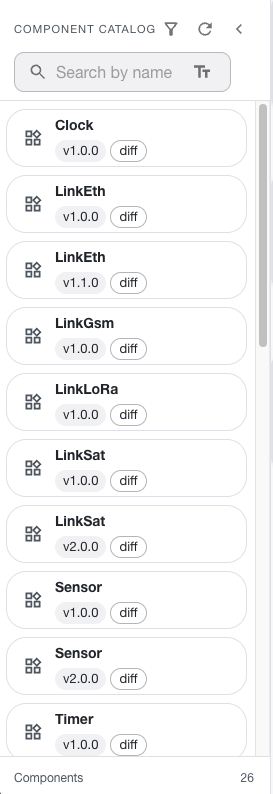
\includegraphics[width=\linewidth,height=0.66\textheight,keepaspectratio]{catalog-panel-1.png}
        \caption{Browse by name.}
        \label{fig:catalog-panel-a}
    \end{subfigure}\hfill
    \begin{subfigure}[t]{0.32\textwidth}
        \centering
        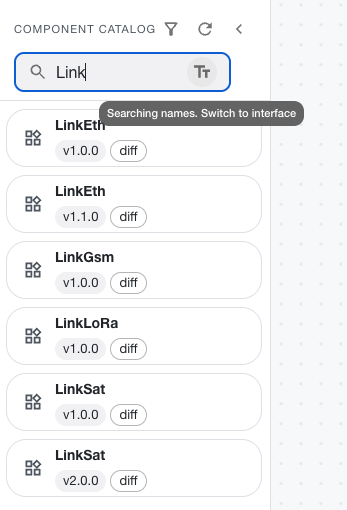
\includegraphics[width=\linewidth,height=0.66\textheight,keepaspectratio]{catalog-panel-2.png}
        \caption{Name search.}
        \label{fig:catalog-panel-b}
    \end{subfigure}\hfill
    \begin{subfigure}[t]{0.32\textwidth}
        \centering
        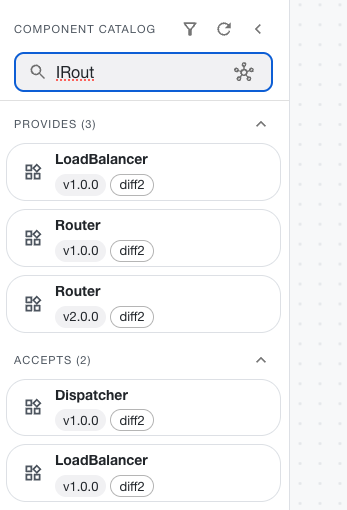
\includegraphics[width=\linewidth,height=0.66\textheight,keepaspectratio]{catalog-panel-3.png}
        \caption{Interface search.}
        \label{fig:catalog-panel-c}
    \end{subfigure}
    \caption[The catalog panel.]{The catalog panel: (a) browsing by name, (b) a name search, (c) an interface search with its provides and accepts grouping.}
    \label{fig:catalog-panel}
\end{figure}

\FloatBarrier

\pagebreak

\subsection{Graph State Management}
\label{sec:graph-state}

The canvas state lives in a Zustand store, \texttt{graphStore}, the renderer's single source of truth for the editable graph. Every change on the canvas ends in a call on this store, which delegates the work to core functions (\S\ref{sec:hex-arch}) and keeps only lifecycle concerns of its own: the dirty flag, the selection sets, and the validator's flagged set. Five small stores share the renderer's state, and two pieces of glue tie them together (Figure~\ref{fig:state-management}).

\begin{figure}[H]
    \centering
    \resizebox{0.92\textwidth}{!}{
        \begin{tikzpicture}[
    font=\small,
    stores/.style={draw, rounded corners=3pt, fill=orange!14, text width=52mm, align=center, minimum height=18mm},
    actor/.style={draw, rounded corners=2pt, text width=34mm, align=center, minimum height=10mm},
    adapter/.style={actor, fill=blue!10},
    view/.style={actor, fill=blue!10},
    orch/.style={actor, fill=green!12},
    subs/.style={actor, fill=yellow!16},
    arr/.style={-{Stealth}, thick},
    lbl/.style={font=\scriptsize, align=center}
]
\node[stores] (stores) {\textbf{Zustand stores}\\[3pt]\scriptsize graphStore\\ catalogStore $\cdot$ workspaceStore\\ uiStore $\cdot$ notificationsStore};

\node[adapter, left=20mm of stores] (adapters) {Adapters\\\scriptsize catalog source, workspace};
\node[view, right=20mm of stores] (view) {Components\\\scriptsize the view};
\node[orch, above=12mm of stores] (cmd) {topologyCommands\\\scriptsize orchestrator};
\node[subs, below=12mm of stores] (sub) {stateSubscriptions};

\draw[arr] (adapters.east) -- node[lbl, above]{write\\outcomes} (stores.west);
\draw[arr] (stores.east) -- node[lbl, above]{select\\slices} (view.west);
\draw[arr] (cmd) -- node[lbl, right]{read graph + workspace,\\ write notifications} (stores);
% Forward and return between stores and subscriptions run as two parallel
% vertical lanes on the lower edge, so they do not overlap.
\draw[arr] ($(stores.south)+(6mm,0)$) -- node[lbl, right]{graph change} ($(sub.north)+(6mm,0)$);
\draw[arr] ($(sub.north)+(-6mm,0)$) -- node[lbl, left, align=center]{prune stale\\ selection /\\ expansion} ($(stores.south)+(-6mm,0)$);
\end{tikzpicture}

    }
    \caption[Renderer state management.]{Renderer state management.}
    \label{fig:state-management}
\end{figure}

\paragraph{The store shape.}
Beyond the graph, the store holds four lifecycle fields (Figure~\ref{fig:graphstore-class}): \texttt{dirty} (the gate UC4 checks), the two selection sets the canvas and the delete hotkey read, and \texttt{flaggedNodeIds} (the validator's snapshot set from \S\ref{sec:validation-engine}).

\begin{figure}[H]
    \centering
    \resizebox{0.95\textwidth}{!}{
        \begin{tikzpicture}[
    font=\small,
    class/.style={draw, rounded corners=1pt, rectangle split, rectangle split parts=3,
        align=left, text width=62mm},
    small/.style={draw, rounded corners=1pt, rectangle split, rectangle split parts=2,
        align=left, text width=50mm, font=\footnotesize},
    comp/.style={{Diamond[length=2.8mm,width=2mm]}-, thick},
    dep/.style={-{Stealth}, thick, dashed},
    lbl/.style={font=\scriptsize\itshape}
]
\node[class] (store) {
    \textbf{GraphStore}\\[1pt]\scriptsize\textit{Zustand store}
    \nodepart{second}
    graph : Graph\\
    dirty : boolean\\
    selectedNodeIds : Set\\
    selectedEdgeIds : Set\\
    flaggedNodeIds : Set
    \nodepart{third}
    setGraph() $\cdot$ markClean()\\
    addNode() $\cdot$ removeNode()\\
    addEdge() $\cdot$ removeEdge()\\
    moveNode() $\cdot$ updateNodeConfig()\\
    renameNode() $\cdot$ removeSelected()\\
    selectNode / selectEdge / selectElements\\
    clearSelection() $\cdot$ setFlaggedNodeIds()
};

\node[small, right=26mm of store.east, yshift=20mm] (graph) {
    \textbf{Graph}
    \nodepart{second}
    nodes : GraphNode[]\\
    edges : GraphEdge[]
};

\node[small, right=26mm of store.east, yshift=-22mm] (ops) {
    \textbf{graphOperations}\\[1pt]\scriptsize\textit{core}
    \nodepart{second}
    addNode(g, n) : Graph\\
    removeNode(g, id) : Graph\\
    addEdge / removeEdge / moveNode\\
    updateNodeConfig / renameNode\\
    validateEdge(g, e) : boolean
};

\draw[comp] (store.east) -- node[lbl, above]{holds} (graph.west);
\draw[dep]  (store.east) -- node[lbl, below]{delegates to} (ops.west);
\end{tikzpicture}

    }
    \caption[The \texttt{graphStore} class.]{The \texttt{graphStore} class}
    \label{fig:graphstore-class}
\end{figure}

\pagebreak

\paragraph{Changes delegate to core functions.}
Every change method in the store is a one-line dispatch: it reads the current graph, hands it to a function in the core that returns the next graph, and writes the next graph back with the dirty flag set. Listing~\ref{lst:store-mutation} shows the pattern, and the same shape repeats for every change. The benefit is that the core function is the only thing the unit tests need to exercise.

\begin{addmargin}[0mm]{0mm}
\begin{lstlisting}[language=, caption={Store action pattern. \texttt{addNode} from the core is a pure function over the graph; the store action wraps it with the lifecycle update.}, label=lst:store-mutation, aboveskip=10pt]
addNode: (node) => set((state) => ({
  graph: addNode(state.graph, node),   // core function
  dirty: true                          // lifecycle concern
})),
\end{lstlisting}
\end{addmargin}


\paragraph{Cascade delete in the core, not in the store.}
Removing a node also removes every edge that references it. Putting the cascade in \texttt{graphOperations.removeNode} (rather than in the store action) keeps the rule unit-testable and reusable. \texttt{removeSelected} is a small generalisation: it walks the two selection sets and applies \texttt{removeNode} or \texttt{removeEdge} for each, then clears the selection.

\paragraph{Reactive subscriptions.}
The store uses Zustand's \texttt{subscribeWithSelector} middleware so \texttt{stateSubscriptions.ts} can react to derived slices: a graph change prunes selection and expansion identifiers that no longer resolve, and a workspace change clears the previous workspace's in-memory state.

\paragraph{Cross-store commands.}
Actions that span stores, such as export (graph, workspace, notification, dirty flag), live in \texttt{src/state/topologyCommands.ts} as plain async functions, so the topbar button and the Ctrl+S hotkey run the same sequence.

\FloatBarrier

\subsection{Canvas Rendering}
\label{sec:canvas-impl}
The canvas is built on React Flow~\cite{react_flow}. React Flow provides the substrate (pannable and zoomable viewport, node and edge primitives, port handles, connection drag visuals, selection box) and lets the application supply custom node and edge components. \texttt{CanvasPanel} is the assembly point: it registers the two custom types and wires every React Flow callback to a store action or a canvas hook, so the component itself holds little logic and the rules stay in the hooks and the core (Figure~\ref{fig:canvas-impl}).

\begin{figure}[H]
    \centering
    \resizebox{0.9\textwidth}{!}{
        \begin{tikzpicture}[
    font=\scriptsize,
    box/.style={draw, rounded corners=2pt, align=center, minimum height=8mm},
    comp/.style={box, fill=blue!10, text width=40mm},
    hook/.style={box, fill=cyan!12, text width=30mm},
    core/.style={box, fill=green!12, text width=58mm},
    store/.style={box, fill=orange!14, text width=40mm},
    arr/.style={-{Stealth}, thick},
    ret/.style={-{Stealth}, thick, dashed},
    lbl/.style={font=\scriptsize\itshape}
]
\node[comp] (panel) {\textbf{CanvasPanel}\\registers node/edge types, wires React Flow callbacks};

\node[hook, below=10mm of panel, xshift=-34mm] (drop) {\textbf{useCatalogDrop}};
\node[hook, below=10mm of panel] (conn) {\textbf{useCanvasConnection}};
\node[hook, below=10mm of panel, xshift=34mm] (keys) {\textbf{useCanvasHotkeys}};

\node[core, below=10mm of conn] (core) {\textbf{Core} (graph, catalog)\\ createNodeFromCatalog \\ validateEdge \\ graphOperations};
\node[store, below=9mm of core] (store) {\textbf{graphStore}};
\node[hook, right=12mm of store] (state) {\textbf{useCanvasState}};

\draw[arr] (panel) -- (drop);
\draw[arr] (panel) -- (conn);
\draw[arr] (panel) -- (keys);
\draw[arr] (drop) -- (core);
\draw[arr] (conn) -- (core);
\draw[arr] (keys) -- (core);
\draw[arr] (core) -- node[lbl, right]{commit} (store);
\draw[arr] (store) -- (state);
\draw[ret] (state.east) -- ++(7mm,0) |- node[lbl, right]{re-render} (panel.east);

\node[lbl, below=7mm of store, text width=92mm, align=center]
    {React Flow event, then hook, then core decision, then store commit. \texttt{useCanvasState} syncs the store back to the view.};
\end{tikzpicture}

    }
    \caption[Canvas components, hooks, core, and store.]{Canvas components and interactions}
    \label{fig:canvas-impl}
\end{figure}

\paragraph{Custom node and edge types.}
React Flow accepts a registry of named node types and edge types; the application uses one of each. \texttt{CanvasNode} renders the instance with input handles on the left, output handles on the right, and, when expanded, three configuration sections. \texttt{CanvasEdge} paints the edge gray by default and red when the validator marks it invalid; a selected edge is blue, and connected ports turn green.

\paragraph{Hooks own the interactions.}
The four interactions from \S\ref{sec:canvas-model} each live in their own hook under \texttt{src/components/canvas/hooks/} (Figure~\ref{fig:canvas-impl}): drop, connection, canvas hotkeys, and the bridge to React Flow's change events. Each is unit-tested with a stub store.

\paragraph{Connection hook.}
\texttt{useCanvasConnection} provides \texttt{isValidConnection} for the in-flight drag and \texttt{onConnect} for the release; both call \texttt{validateEdge} from \texttt{graphOperations.ts}, the single source of truth for what a valid edge is. An endpoint dropped on empty space deletes the edge rather than leaving it dangling.

\paragraph{Edit hook and node sections.}
An expanded node shows three sections (info, requirements, configuration); a per-type control renderer applies the per-field input constraints (\S\ref{sec:validation-impl}) and feeds each edit to \texttt{graphStore.updateNodeConfig}.

\begin{figure}[H]
    \centering
    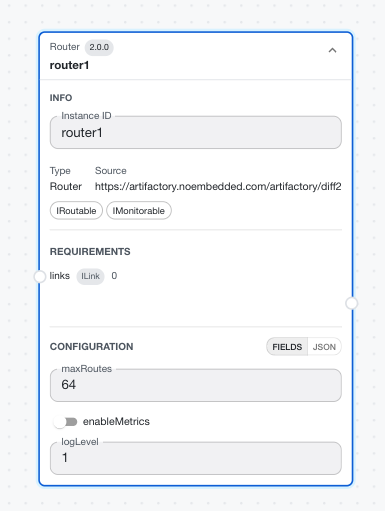
\includegraphics[width=0.45\linewidth,keepaspectratio]{node-expand.png}
    \caption[An expanded node on the canvas.]{An expanded node, showing the three sections and inline typed configuration fields.}
    \label{fig:canvas-expanded-node}
\end{figure}

\paragraph{Hotkey hook and focus discipline.}
\texttt{useCanvasHotkeys} installs a window-scope keydown listener and skips its handlers when the active element is a text input, so typing a digit into a configuration field does not also delete the node. The app-scope hotkey hook carries the same guard; the full key bindings are listed in \S\ref{sec:hotkeys}.

\FloatBarrier

\subsection{Topology Export and Import}
\label{sec:topology-impl}
Export and import are two core functions over the same data model, with thin adapters that wire them to the IPC layer. They are the only places where the graph representation and the wire representation meet. Figure~\ref{fig:domain-classes} is the data model, the graph on the left and the topology on the right; Figure~\ref{fig:topology-functions} is the step sequence each function runs.

\clearpage
\begin{figure}[H]
    \centering
    \resizebox{0.96\textwidth}{!}{
        \begin{tikzpicture}[
    font=\scriptsize,
    class/.style={draw, rectangle split, rectangle split parts=2, fill=blue!8, text width=38mm, align=left},
    tcls/.style={draw, rectangle split, rectangle split parts=2, fill=orange!10, text width=38mm, align=left},
    comp/.style={{Diamond[open]}-, thick},
    trans/.style={-{Stealth}, dashed, thick},
    lbl/.style={font=\scriptsize\itshape, align=center}
]
\node[class] (graph) {\textbf{Graph}
    \nodepart{two} nodes: GraphNode[]\\ edges: GraphEdge[]};
\node[class, below left=14mm and -14mm of graph] (gnode) {\textbf{GraphNode}
    \nodepart{two} id, instanceId\\ componentType, version\\ position, configData\\ slots: Slot[]};
\node[class, below right=14mm and -14mm of graph] (gedge) {\textbf{GraphEdge}
    \nodepart{two} id\\ sourceNodeId, sourceSlot\\ targetNodeId, targetSlot};
\node[class, below=12mm of gnode] (slot) {\textbf{Slot}
    \nodepart{two} name, type\\ direction, isArray};

\node[tcls, right=42mm of graph] (topo) {\textbf{Topology}
    \nodepart{two} entries: TopologyEntry[]};
\node[tcls, below=16mm of topo] (entry) {\textbf{TopologyEntry}
    \nodepart{two} type, id\\ dependencies:\\ \quad(string $|$ string[])[]\\ config};

\draw[comp] (graph) -- (gnode);
\draw[comp] (graph) -- (gedge);
\draw[comp] (gnode) -- (slot);
\draw[comp] (topo) -- (entry);

\draw[trans] ($(graph.east)+(0,3mm)$) -- node[lbl, above]{graphToTopology\\(Kahn order)} ($(topo.west)+(0,3mm)$);
\draw[trans] ($(topo.west)+(0,-3mm)$) -- node[lbl, below]{topologyToGraph\\(+ auto-layout)} ($(graph.east)+(0,-3mm)$);

\end{tikzpicture}

    }
    \caption[The graph and topology data model.]{The graph and topology data model.}
    \label{fig:domain-classes}
\end{figure}

\begin{figure}[H]
    \centering
    \begin{subfigure}{\textwidth}
        \centering
        \resizebox{0.7\textwidth}{!}{\begin{tikzpicture}[
    font=\scriptsize,
    head/.style={draw, rounded corners=2pt, fill=white, text width=30mm, minimum height=10mm, align=center, anchor=north},
    life/.style={dashed, gray},
    call/.style={-{Stealth}, thick},
    ret/.style={-{Stealth}, thick, dashed},
    msg/.style={font=\scriptsize, align=center, fill=white, inner sep=1pt},
    frame/.style={draw, thick},
    ftag/.style={draw, thick, fill=white, font=\scriptsize\bfseries, inner sep=2pt, anchor=north west}
]
\def\sp{44mm}
\node[head] (gt) at (0,0) {\texttt{graphToTopology}};
\node[head] (ks) at (\sp,0) {Kahn topo-sort};
\node[head] (df) at (2*\sp,0) {\texttt{depsFor}};
\def\botY{-56mm}
\foreach \n in {gt,ks,df}{\draw[life] (\n.south) -- (\n.south |- 0,\botY);}

\def\rA{-17mm}\def\rB{-25mm}\def\loopT{-31mm}\def\rC{-40mm}\def\rD{-48mm}\def\loopB{-52mm}

\draw[call] (gt.center |- 0,\rA) -- node[msg,above]{order by dependency} (ks.center |- 0,\rA);
\draw[ret]  (ks.center |- 0,\rB) -- node[msg,above]{nodes in dependency order} (gt.center |- 0,\rB);

\draw[frame] (-12mm,\loopT) rectangle (2*\sp+12mm,\loopB);
\node[ftag] at (-12mm,\loopT) {loop [per node]};
\draw[call] (gt.center |- 0,\rC) -- node[msg,above]{align deps to slot order} (df.center |- 0,\rC);
\draw[ret]  (df.center |- 0,\rD) -- node[msg,above]{dependency list} (gt.center |- 0,\rD);

\node[msg, anchor=north west] at (-12mm,\botY) {result: the dependency-ordered \texttt{Topology}};
\end{tikzpicture}
}
        \caption{Export: \texttt{graphToTopology}.}
        \label{fig:topology-functions-export}
    \end{subfigure}\\[6pt]
    \begin{subfigure}{\textwidth}
        \centering
        \resizebox{0.7\textwidth}{!}{\begin{tikzpicture}[
    font=\scriptsize,
    head/.style={draw, rounded corners=2pt, fill=white, text width=32mm, minimum height=10mm, align=center, anchor=north},
    life/.style={dashed, gray},
    call/.style={-{Stealth}, thick},
    ret/.style={-{Stealth}, thick, dashed},
    msg/.style={font=\scriptsize, align=center, fill=white, inner sep=1pt},
    frame/.style={draw, thick},
    ftag/.style={draw, thick, fill=white, font=\scriptsize\bfseries, inner sep=2pt, anchor=north west}
]
\def\sp{46mm}
\node[head] (tg) at (0,0) {\texttt{topologyToGraph}};
\node[head] (cb) at (\sp,0) {catalog + \texttt{buildSlots}};
\node[head] (ll) at (2*\sp,0) {\texttt{layoutByLevels}};
\def\botY{-71mm}
\foreach \n in {tg,cb,ll}{\draw[life] (\n.south) -- (\n.south |- 0,\botY);}

\def\rPa{-16mm}\def\rPb{-22mm}\def\loopT{-28mm}\def\rC{-37mm}\def\rD{-45mm}\def\loopB{-50mm}
\def\rE{-58mm}\def\rF{-66mm}

% self-call: parse + shape-check
\draw[call] (tg.center |- 0,\rPa) -- ++(7mm,0) |- (tg.center |- 0,\rPb);
\node[msg, anchor=west] at ($(tg.center |- 0,\rPa)+(9mm,-3mm)$) {parse + shape-check};

% loop [per entry]
\draw[frame] (-12mm,\loopT) rectangle (\sp+14mm,\loopB);
\node[ftag] at (-12mm,\loopT) {loop [per entry]};
\draw[call] (tg.center |- 0,\rC) -- node[msg,above]{lookup type, build slots} (cb.center |- 0,\rC);
\draw[ret]  (cb.center |- 0,\rD) -- node[msg,above]{node skeleton} (tg.center |- 0,\rD);

% layout, after the loop
\draw[call] (tg.center |- 0,\rE) -- node[msg,above]{place by depth} (ll.center |- 0,\rE);
\draw[ret]  (ll.center |- 0,\rF) -- node[msg,above]{positions} (tg.center |- 0,\rF);

\node[msg, anchor=north west] at (-12mm,\botY) {result: the reconstructed \texttt{Graph}};
\end{tikzpicture}
}
        \caption{Import: \texttt{topologyToGraph}.}
        \label{fig:topology-functions-import}
    \end{subfigure}
    \caption[The export and import function pipelines.]{The step sequence each function runs. (a) \texttt{graphToTopology} orders the graph and aligns each node's dependencies to its slots; (b) \texttt{topologyToGraph} parses the file and rebuilds each node from the catalog.}
    \label{fig:topology-functions}
\end{figure}

\pagebreak

\paragraph{Export.}
\texttt{graphToTopology} emits the entries in dependency order with Kahn's algorithm (\S2.2.1), breaking ties by the node's original order so the output is deterministic. Each entry's dependency list comes from \texttt{depsFor}.

\paragraph{}
A topology entry's \texttt{dependencies} field aligns one-to-one with the component's declared input slots. For a non-array slot the entry is the source instance identifier; for an array slot the entry is a JSON array of identifiers (Listing~\ref{lst:depsfor}). The alignment lets the C++ constructor receive the right interface in the right argument position without parsing slot names at runtime. Empty array slots emit an empty array; unfilled non-array slots emit an empty string, which the structural validator catches at export time before \texttt{graphToTopology} is called.

\begin{addmargin}[0mm]{0mm}
\begin{lstlisting}[language=, caption={\texttt{depsFor}. Walks the component's declared input slots in order and emits one slot value per position.}, label=lst:depsfor, aboveskip=10pt]
function depsFor(node, incomingEdges, nodeMap): TopologyDependency[] {
  const inSlots = node.slots.filter(s => s.direction === 'in')
  const bySlot = groupBy(incomingEdges.get(node.id) ?? [], e => e.targetSlot)
  return inSlots.map(slot => {
    const ids = (bySlot.get(slot.name) ?? []).map(e => nodeMap.get(e.sourceNodeId)?.instanceId)
    return slot.isArray ? ids : (ids[0] ?? '')
  })
}
\end{lstlisting}
\end{addmargin}

\paragraph{Import.}
\texttt{topologyToGraph} reverses the operation: it rebuilds each node (type lookup, \texttt{buildSlots}, config copy) and seeds positions from \texttt{layoutByLevels}, which places nodes by topological depth so the graph reads left to right as node positions are not carried by the format.

\paragraph{}
\texttt{topologyToGraph} still returns a node when the entry's type is missing from the catalog. The canvas marks it unresolved at render time, finding no catalog entry for the node's type, and draws it in a dashed red frame with a warning, the behaviour motivated in \S\ref{sec:topology-io}.

\FloatBarrier

\subsection{Validation Engine}
\label{sec:validation-impl}

The two-phase design from \S\ref{sec:validation-engine} splits across two layers. The per-field phase is enforced at the configuration controls as the integrator types, and \texttt{updateNodeConfig} merges the committed value into the node. The structural phase lives in \texttt{validateGraph} under \texttt{core/graph}, triggers only at export time, and returns a flat result that the canvas uses to paint flagged nodes.

\paragraph{Per-field validation lives on the node.}
The per-field phase is constraint-based rather than a validation pass. \texttt{ConfigFieldRenderer} picks a control by the field's declared type: a numeric field renders an HTML number input carrying the type's range and step (the signed or unsigned integer bounds, or \texttt{step=any} for \texttt{float} and \texttt{double}), tightened by any \texttt{min} or \texttt{max} the schema declares; a string field caps its length with \texttt{maxLength}; a boolean renders a switch. The control constrains the value at entry, and \texttt{updateNodeConfig} commits a numeric edit only when it parses as a number, so an out-of-type value never reaches \texttt{configData}. There is no separate per-field error state; the structural validator below is the gate that blocks export.

\paragraph{Structural result shape.}
\texttt{validateGraph} returns a \texttt{GraphValidationResult}: a \texttt{valid} boolean plus three lists, one per failure class (Listing~\ref{lst:validation-result}). The shape is flat and serialisable, which makes the failure data round-trip through the renderer toast and the flagged-node set.

\begin{addmargin}[0mm]{0mm}
\begin{lstlisting}[language=, caption={The validation result. \texttt{cycles[i]} is a list of node identifiers forming the cycle; \texttt{unfilled[i]} carries the offending node and slot; \texttt{invalidEdges[i]} is the edge identifier.}, label=lst:validation-result, aboveskip=10pt]
type UnfilledSlot = { 
  nodeId: string; 
  instanceId: string; 
  slotName: string 
}

type GraphValidationResult = {
  valid:        boolean
  cycles:       string[][]
  unfilled:     UnfilledSlot[]
  invalidEdges: string[]
}
\end{lstlisting}
\end{addmargin}

\begin{figure}[H]
    \centering
    \resizebox{0.8\textwidth}{!}{
        \begin{tikzpicture}[
    font=\scriptsize,
    fn/.style={draw, rounded corners=2pt, fill=green!12, text width=40mm, align=center, minimum height=8mm},
    caller/.style={draw, rounded corners=2pt, fill=blue!10, text width=34mm, align=center, minimum height=8mm},
    data/.style={draw, rectangle split, rectangle split parts=2, fill=yellow!14, text width=44mm, align=left},
    ui/.style={draw, rounded corners=2pt, fill=orange!14, text width=40mm, align=center, minimum height=8mm},
    arr/.style={-{Stealth}, thick},
    ret/.style={-{Stealth}, thick, dashed},
    lbl/.style={font=\scriptsize\itshape, align=center}
]
\node[caller] (export) {exportTopology (command)};
\node[fn, below=8mm of export] (vg) {validateGraph};
\node[fn, below=11mm of vg, xshift=-46mm] (cyc) {detectCycles};
\node[fn, below=11mm of vg] (unf) {detectUnfilled-\\RequiredSlots};
\node[fn, below=11mm of vg, xshift=46mm] (edge) {isEdgeInvalid\\(per edge)};
\node[data, below=11mm of unf] (res) {\textbf{GraphValidationResult}
    \nodepart{two} valid: bool\\ cycles, unfilled, invalidEdges};
\node[ui, below=9mm of res] (flag) {flaggedNodeIds: red node borders};

\draw[arr] (export) -- node[lbl, right]{at export} (vg);
\draw[arr] (vg) -- (cyc);
\draw[arr] (vg) -- (unf);
\draw[arr] (vg) -- (edge);
\draw[arr] (cyc) -- (res.north west);
\draw[arr] (unf) -- (res.north);
\draw[arr] (edge) -- (res.north east);
\draw[ret] (res.east) -| node[lbl, right, pos=0.25]{valid: write file;\\ invalid: refuse} ($(edge.east)+(8mm,0)$) |- (export.east);
\draw[arr] (res) -- node[lbl, right]{on failure} (flag);
\end{tikzpicture}

    }
    \caption[How the structural validator composes.]{\texttt{validateGraph} runs three detectors, aggregates a single result, and the export command either writes the file or refuses it and flags the offending nodes.}
    \label{fig:validation-impl}
\end{figure}

\paragraph{}
Cycles are found by a depth-first search that keeps a recursion stack. When an edge reaches a node already on the stack, the path back to it is a cycle, rebuilt from the parent pointers kept during the descent; the search is linear and reports one entry per distinct cycle. Export reuses Kahn's algorithm only for ordering, so the dedicated search is what yields the actual cycle members Kahn does not surface.

\paragraph{}
\texttt{detectUnfilledRequiredSlots} counts incoming edges per (node, slot) pair, then reports the non-array slots whose count is zero. Array slots are deliberately excluded; an empty array is valid (the C++ side accepts a zero-length variadic). The result names the offending instance identifier rather than the internal node id.

\paragraph{}
The connection-time validator in \S\ref{sec:canvas-impl} rejects an invalid edge before it enters the graph. \texttt{validateGraph} re-checks every edge with \texttt{isEdgeInvalid} at export time anyway, catching an edge that became invalid through some other path, such as a catalog refresh that changed a slot's interface. The benefit is that the loader downstream of \texttt{diff-forge} never sees a structurally invalid edge.

\paragraph{}
On a failed export the command unions the node identifiers named by the three failure lists and hands the set to \texttt{graphStore.setFlaggedNodeIds}; the canvas paints those nodes. The set is pruned (never grown) on node removal and on \texttt{setGraph}, and a fresh export recomputes it. This ties the visual feedback to the last real validation decision without re-running cycle detection on every keystroke, which would put NFR-1.2 out of reach on a fifty-node graph.

\begin{figure}[H]
    \centering
    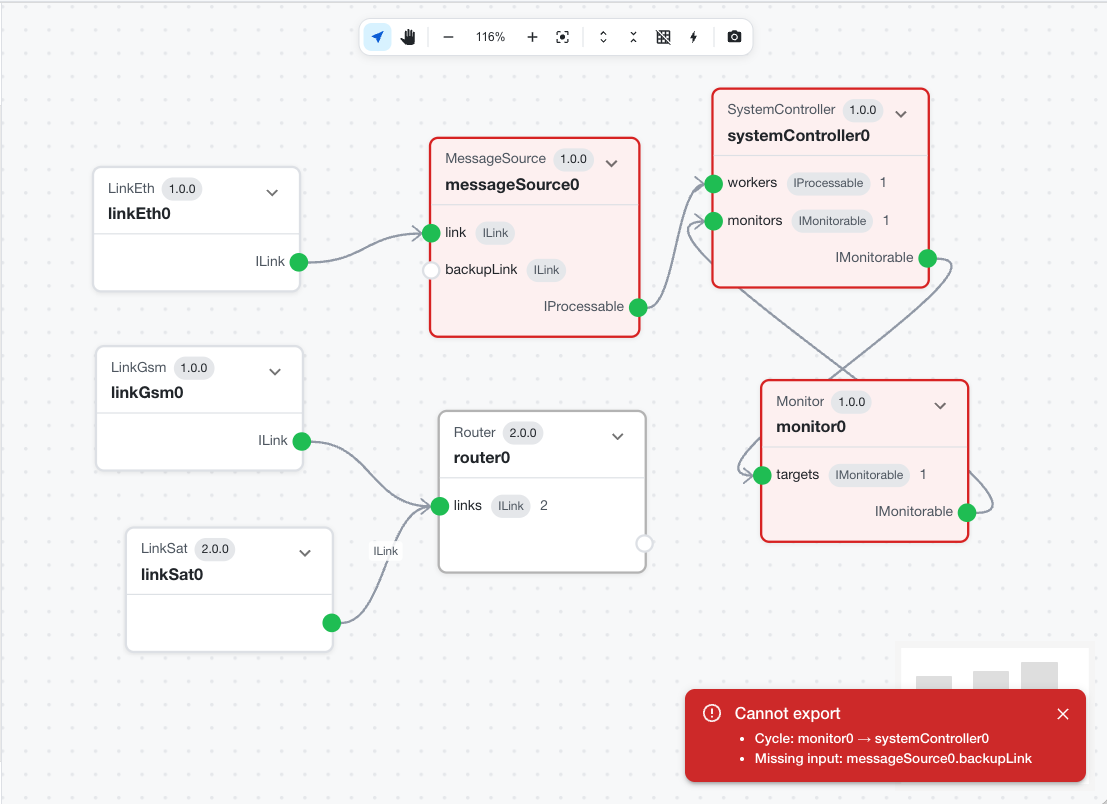
\includegraphics[width=0.8\linewidth,height=0.5\textheight,keepaspectratio]{validation-flagged.png}
    \caption[Flagged nodes after a blocked export.]{Nodes flagged by the structural validator after a blocked export.}
    \label{fig:validation-flagged}
\end{figure}

\FloatBarrier

\subsection{Workspace Flow and User Interface}
\label{sec:workspace-ui}

\texttt{App.tsx} is the renderer root. It wires three boot effects, picks the layout based on their results, and renders the global UI shell (Backdrop, toast host, hotkey hook). All three effects fire concurrently and the layout choice is the conjunction of "catalog is usable" and "workspace is valid".

\begin{itemize}
    \item The catalog effect calls \texttt{ipcCatalogSource.loadCatalog()} and writes the outcome to \texttt{catalogStore.setStatus}.
    \item The workspace effect calls \texttt{ipcWorkspaceStore.getStatus()} and writes the outcome to \texttt{workspaceStore.setStatus}.
    \item The topology effect waits for both to become \textit{ready}, then calls \\ \texttt{ipcWorkspaceStore.loadTopology()}, parses the result through \texttt{parseTopology}, reconstructs the graph, and writes it to \texttt{graphStore.setGraph}. The \texttt{lastLoadedCwd} ref gates the load on the workspace \texttt{cwd} differing from the last one loaded, so a stale catalog update cannot re-run the load and discard an in-progress edit.
\end{itemize}

\begin{figure}[H]
    \centering
    \resizebox{0.82\textwidth}{!}{
        \begin{tikzpicture}[
    font=\scriptsize,
    app/.style={draw, rounded corners=2pt, fill=blue!10, text width=42mm, align=center, minimum height=8mm},
    effect/.style={draw, rounded corners=2pt, fill=green!12, text width=44mm, align=center, minimum height=8mm},
    layout/.style={draw, rounded corners=2pt, fill=orange!14, text width=40mm, align=center, minimum height=8mm},
    dec/.style={diamond, draw, aspect=2.6, inner sep=1pt, fill=yellow!18, align=center, font=\scriptsize},
    arr/.style={-{Stealth}, thick},
    lbl/.style={font=\scriptsize\itshape}
]
\node[app] (app) {App.tsx (renderer root)};
\node[effect, below=9mm of app, xshift=-32mm] (a) {Effect A: load catalog\\ into catalogStore};
\node[effect, below=9mm of app, xshift=32mm] (b) {Effect B: workspace status\\ into workspaceStore};
\node[dec, below=10mm of app, yshift=-12mm] (ready) {catalog usable\\ and workspace valid?};
\node[layout, below=10mm of ready, xshift=-34mm] (welcome) {InitialLayout\\ welcome: pick workspace,\\ retry catalog};
\node[layout, below=10mm of ready, xshift=34mm] (main) {MainLayout (editor)};
\node[effect, below=9mm of main] (c) {Effect C: load topology,\\ topologyToGraph into graphStore};

\draw[arr] (app) -- node[lbl, left]{concurrent} (a);
\draw[arr] (app) -- (b);
\draw[arr] (a) -- (ready);
\draw[arr] (b) -- (ready);
\draw[arr] (ready) -- node[lbl, above left]{no} (welcome);
\draw[arr] (ready) -- node[lbl, above right]{yes} (main);
\draw[arr] (main) -- node[lbl, right]{on first ready} (c);
\end{tikzpicture}

    }
    \caption[The boot sequence.]{The boot sequence. Effects A and B run concurrently; the layout is the welcome screen until both the catalog and the workspace are ready, after which the editor mounts and Effect C loads the topology.}
    \label{fig:boot}
\end{figure}

\paragraph{The two layouts.}
\texttt{MainLayout} is the editing surface: a fixed-width left column with the catalog panel, the canvas filling the rest, and a topbar across the top. \texttt{InitialLayout} is the welcome surface: a centered card with two sections, one per readiness signal that has not flipped to ready. \texttt{CatalogSection} surfaces the catalog status and a Retry that re-triggers \texttt{loadCatalog}. \texttt{WorkspaceSection} surfaces the reason the workspace is invalid and a folder picker; the user can also type a path, routed through \texttt{workspace.openAtPath}.

\begin{figure}[H]
    \centering
    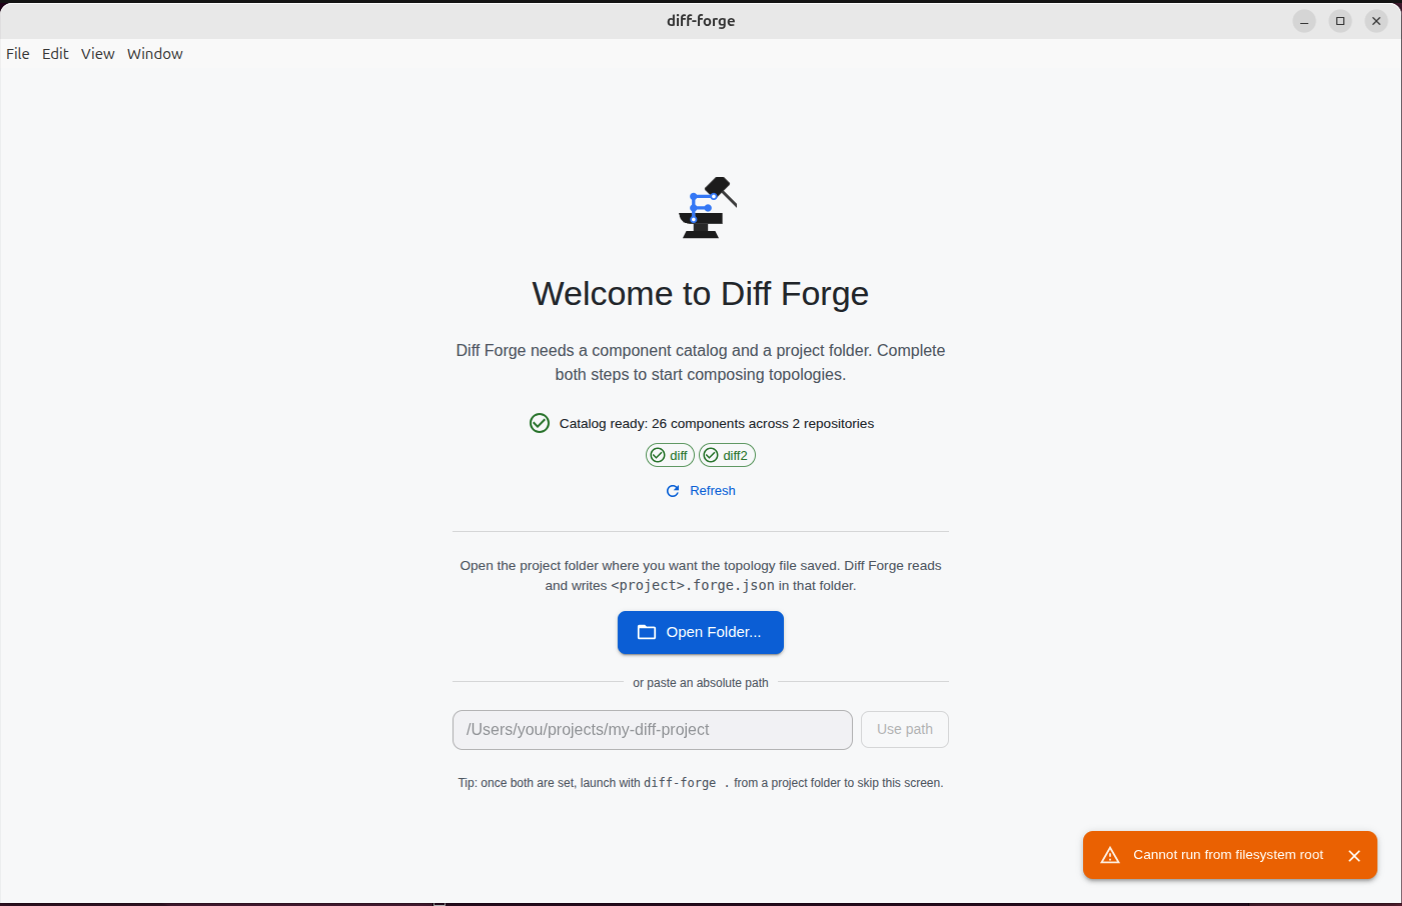
\includegraphics[width=0.8\linewidth,height=0.5\textheight,keepaspectratio]{welcome.png}
    \caption[The welcome screen.]{The welcome screen, shown until both the workspace and the catalog are ready.}
    \label{fig:welcome}
\end{figure}

\paragraph{Topbar.}
The topbar carries the workspace chip (clickable, opens the picker via the same command that the Ctrl+O hotkey runs), a Save Topology button (calls \texttt{exportTopology}, disabled when the workspace is invalid), a help icon (opens an About dialog), and a keyboard icon (opens the hotkey reference dialog).

\paragraph{Dirty-aware workspace switch.}
\texttt{topologyCommands.requestWorkspaceSwitch} reads \texttt{graphStore.dirty}. If false, it falls straight through to \texttt{performWorkspaceSwitch}. If true, it opens a confirmation dialog, and only switches workspace once the user confirms. \texttt{performWorkspaceSwitch} opens the native picker, and on success writes the new status to the store. The cwd change is observed by the topology effect, which re-runs and reconstitutes the new workspace's graph.

\paragraph{Notifications.}
\texttt{notificationsStore} is a small Zustand store holding a list of toast records (id, severity, message, timeout). Free \texttt{notify.*} helpers push a record and schedule its removal, and \texttt{NotificationHost} renders the list as a stack of Material UI (MUI) \texttt{Snackbar}s in the bottom-right corner. Most user actions end in exactly one toast; the queue exists so a multi-step action does not lose the earlier message.

\begin{figure}[H]
    \centering
    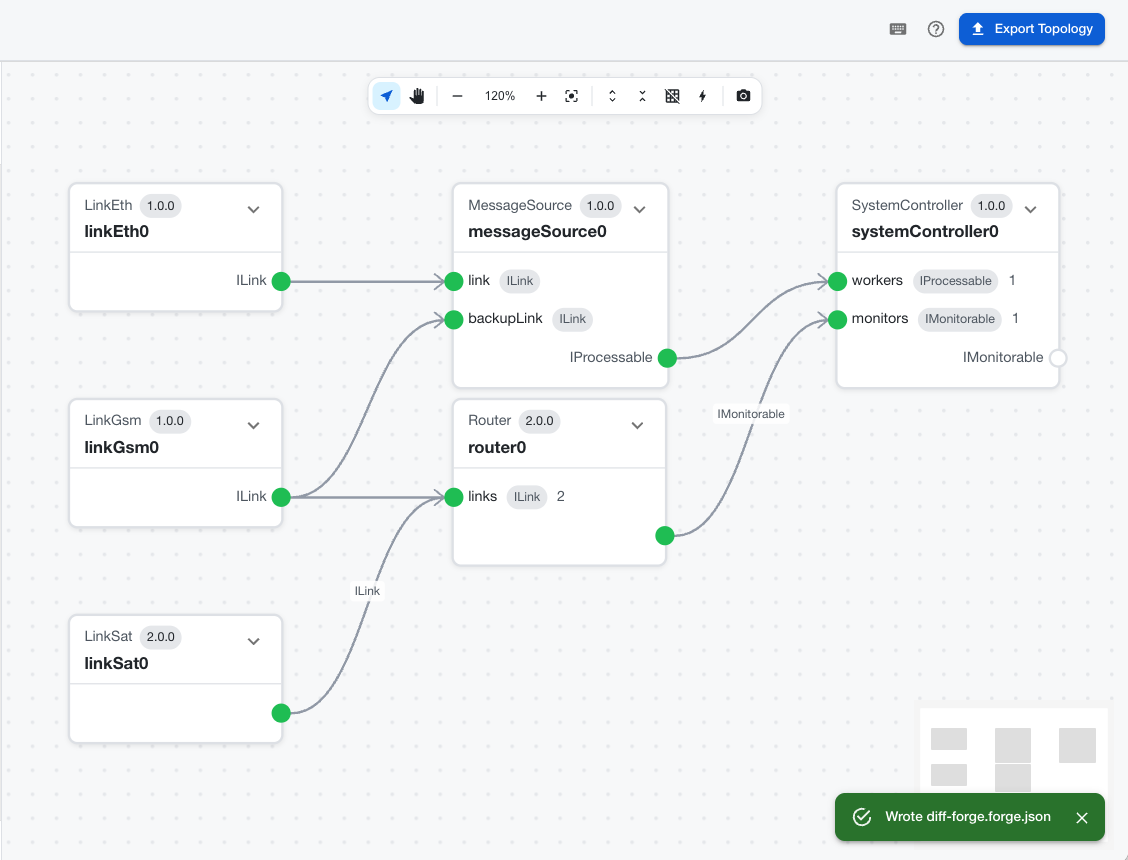
\includegraphics[width=0.6\linewidth,keepaspectratio]{export-toast.png}
    \caption[Export feedback toast.]{The toast shown after n success export.}
    \label{fig:export-toast}
\end{figure}

\paragraph{Keyboard bindings.}
\label{sec:hotkeys}
Every authoring action reachable with the mouse is also reachable from the keyboard (NFR-3.1), and a reference dialog opened from the topbar lists the bindings (NFR-3.3). The bindings use \texttt{Ctrl} on every platform, with no per-operating-system remapping. Table~\ref{tab:hotkeys} lists them, and the reference dialog renders from the same binding list, so the documentation cannot drift from the behaviour.

\begin{table}[H]
\centering
\caption[Keyboard bindings.]{Keyboard bindings. The same key is used on every platform.}
\label{tab:hotkeys}
\footnotesize
\begin{tabular}{ll}
\toprule
\textbf{Key} & \textbf{Action} \\
\midrule
\texttt{Ctrl+S}             & Export the topology \\
\texttt{Ctrl+O}             & Open or switch the workspace \\
\texttt{Ctrl+A}             & Select every node and edge \\
\texttt{Delete} / \texttt{Backspace} & Delete the current selection \\
\texttt{Space} (hold)       & Temporarily pan the canvas \\
\bottomrule
\end{tabular}
\end{table}

The bindings stand down while a text input has focus (\S\ref{sec:canvas-impl}), so editing a configuration field never triggers a shortcut.

\begin{figure}[H]
    \centering
    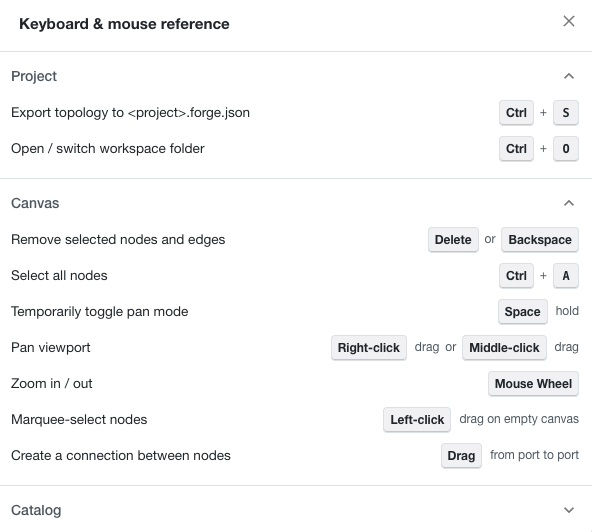
\includegraphics[width=0.6\linewidth,keepaspectratio]{hotkey.png}
    \caption[The hotkey reference dialog.]{The hotkey reference dialog, reachable from the topbar without leaving the editor.}
    \label{fig:hotkey-dialog}
\end{figure}

\FloatBarrier

\input{tex/6-evaluation}
\input{tex/7-conclusion}

%-------------------------
% Bibliography
%-------------------------
\cleardoublepage
\printbibliography
\clearpage

%-------------------------
% Symbols and Abbreviations
%-------------------------
\acronymlist
\acronym{EiTI}{Faculty of Electronics and Information Technology}
\acronym{WUT}{Warsaw University of Technology}
\acronym{DI}{Dependency Injection}
\acronym{IAiIS}{Institute of Control and Computation Engineering}
\acronym{CBSE}{Component-Based Software Engineering}
\acronym{GUI}{Graphical User Interface}
\vspace{0.8cm}

%-------------------------
% Lists: Figures, Tables, Appendices
%-------------------------
\pagestyle{plain}

\listoffigurestoc
\vspace{1cm}
\listoftablestoc
\vspace{1cm}
\listofappendicestoc

%-------------------------
% Appendices
%-------------------------
\captionsetup[figure]{list=no}
\captionsetup[table]{list=no}

\clearpage
\appendix{User Manual}
Instructions for installing and running \texttt{diff-forge}.

\clearpage
\appendix{Configuration Schema}
The JSON schema used for component metadata.

\end{document}
